\documentclass[11pt]{article}
\usepackage[margin=1.05in]{geometry}
\usepackage{amsmath,amssymb,amsthm}
\usepackage{booktabs,array,longtable}
\usepackage{tikz}
\usepackage{xcolor}
\usepackage{graphicx}
\usepackage[hidelinks]{hyperref}
\usepackage{caption}
\captionsetup{font=small,labelfont=bf}

\newtheorem{theorem}{Theorem}
\newtheorem{proposition}[theorem]{Proposition}
\newtheorem{lemma}[theorem]{Lemma}
\newtheorem{corollary}[theorem]{Corollary}
\newtheorem{question}[theorem]{Question}
\theoremstyle{definition}
\newtheorem{definition}[theorem]{Definition}
\theoremstyle{remark}
\newtheorem{remark}[theorem]{Remark}
\newtheorem{example}[theorem]{Example}

\newcommand{\R}{\mathbb{R}}
\newcommand{\Z}{\mathbb{Z}}
\newcommand{\Dir}{\R/2\pi\Z}
\newcommand{\vstar}{v_\ast}
\newcommand{\hid}[1]{\bar{#1}}

\definecolor{cA}{HTML}{8F96A3}
\definecolor{cP1}{HTML}{F28E2B}
\definecolor{cP2}{HTML}{B07AA1}
\definecolor{cP3}{HTML}{D2AA16}
\definecolor{cI}{HTML}{8C564B}
\definecolor{cF}{HTML}{4FA34A}
\definecolor{cC}{HTML}{138A82}
\definecolor{cCp}{HTML}{EF6FA6}
\definecolor{cE}{HTML}{6A51A3}
\definecolor{cEp}{HTML}{5FB0E8}
\tikzset{
  mtn/.style={red!70!black,line width=0.7pt,dash pattern=on 4pt off 1.2pt on 0.8pt off 1.2pt},
  val/.style={blue!65!black,line width=0.7pt,dash pattern=on 3pt off 1.6pt},
  refl/.style={black!55,line width=0.5pt,dash pattern=on 0.6pt off 1.4pt},
  sheet/.style={line width=0.8pt},
  crease/.style={line width=0.6pt},
  ch/.style={line width=2.1pt,line cap=round,opacity=0.85},
  virt/.style={line width=0.6pt,double distance=1.6pt,dash pattern=on 2pt off 1.5pt},
}

\title{Reading the folding history of a crease pattern\\ from local histories at its vertices}
\author{}
\date{October 16, 2026}

\begin{document}
\maketitle

\begin{abstract}
A crease pattern records where a sheet was folded but not in what order. We give a method that recovers much of the order from the pattern alone, and test it on a corpus of published patterns. Its central object is the \emph{local history} at a vertex: a sequence of folds, each through one line in the folded paper, that produces the creases at that vertex. We show that, apart from a collision test, local histories are characterised by two conditions on the creases made at one time: there is an even number of them, and any two are related by the product of reflections in the earlier creases lying between them. The product has a closed form, an alternating sum of directions, so the condition is linear once the set of earlier creases is fixed. Creases that were made and later erased are recovered as cancelled segments, which must themselves have local histories wherever they cross the pattern; moves that fold several lines at once are admitted at a cost. Requiring one order of all creases to be consistent with a local history at every vertex yields a constraint problem, which we solve with an SMT solver. The output partitions the creases into \emph{folds}, sets of creases that must be made together, and orders the folds partially. We work two small patterns by hand and a $278$-crease dragon by machine; on $48$ patterns from a public collection, $42$ are resolved, and the rest mark where the method stops.
\end{abstract}

\begin{figure}[t]
\centering
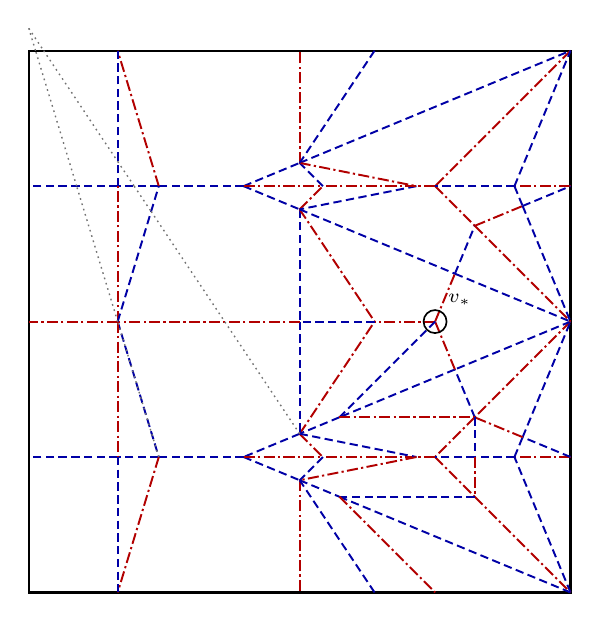
\begin{tikzpicture}[x=0.86cm,y=0.86cm]
\draw[sheet] (0,0) rectangle (8,8);
\draw[mtn] (8,6) -- (7.172,6);
\draw[mtn] (8,2) -- (7.172,2);
\draw[mtn] (6,2) -- (6.586,1.414);
\draw[mtn] (6,2) -- (5.725,2);
\draw[mtn] (8,4) -- (6.586,2.586);
\draw[mtn] (6,6) -- (6.586,5.414);
\draw[mtn] (6,6) -- (5.725,6);
\draw[mtn] (8,8) -- (6,6);
\draw[val] (3.172,6) -- (4,6.343);
\draw[val] (3.172,6) -- (1.92,6);
\draw[val] (3.172,2) -- (4,1.657);
\draw[val] (3.172,2) -- (1.92,2);
\draw[val] (3.172,6) -- (4,5.657);
\draw[val] (7.172,2) -- (7.293,2.293);
\draw[val] (7.172,2) -- (6.586,2);
\draw[val] (8,0) -- (7.172,2);
\draw[val] (7.172,6) -- (7.293,5.707);
\draw[val] (7.172,6) -- (6,6);
\draw[val] (7.172,6) -- (8,8);
\draw[val] (4,6.343) -- (8,8);
\draw[val] (4,1.657) -- (4.586,1.414);
\draw[val] (4,2.343) -- (3.172,2);
\draw[mtn] (4,5.657) -- (4.343,6);
\draw[val] (4.343,6) -- (4,6.343);
\draw[mtn] (4,6.343) -- (4,8);
\draw[val] (4,5.657) -- (4,4);
\draw[mtn] (4,2.343) -- (4.343,2);
\draw[val] (4.343,2) -- (4,1.657);
\draw[mtn] (4,1.657) -- (4,0);
\draw[mtn] (3.172,2) -- (4.343,2);
\draw[mtn] (3.172,6) -- (4.343,6);
\draw[mtn] (4,2.343) -- (5.107,4);
\draw[mtn] (4,5.657) -- (5.107,4);
\draw[val] (5.107,4) -- (4,4);
\draw[val] (4,4) -- (4,2.343);
\draw[val] (8,4) -- (6.293,3.293);
\draw[val] (4,5.657) -- (6.293,4.707);
\draw[mtn] (4,4) -- (1.313,4);
\draw[val] (5.725,6) -- (4,5.657);
\draw[mtn] (5.725,6) -- (4.343,6);
\draw[mtn] (4,6.343) -- (5.725,6);
\draw[val] (5.107,8) -- (4,6.343);
\draw[mtn] (5.725,2) -- (4.343,2);
\draw[val] (4,2.343) -- (5.725,2);
\draw[mtn] (5.725,2) -- (4,1.657);
\draw[val] (5.107,0) -- (4,1.657);
\draw[val] (1.313,4) -- (1.92,2);
\draw[val] (1.92,2) -- (1.313,2);
\draw[mtn] (1.313,4) -- (0,4);
\draw[mtn] (1.92,2) -- (1.313,0);
\draw[val] (1.92,6) -- (1.313,6);
\draw[mtn] (1.92,6) -- (1.313,8);
\draw[val] (1.313,2) -- (0,2);
\draw[val] (1.313,6) -- (0,6);
\draw[mtn] (1.313,4) -- (1.313,6);
\draw[val] (1.313,6) -- (1.313,8);
\draw[mtn] (1.313,4) -- (1.313,2);
\draw[val] (1.313,2) -- (1.313,0);
\draw[val] (7.293,2.293) -- (8,4);
\draw[val] (8,2) -- (7.293,2.293);
\draw[mtn] (7.293,2.293) -- (6.586,2.586);
\draw[mtn] (6.586,2.586) -- (6,2);
\draw[val] (6.586,2.586) -- (6.293,3.293);
\draw[val] (6.293,3.293) -- (4.586,2.586);
\draw[mtn] (6.293,3.293) -- (6,4);
\draw[mtn] (6,4) -- (5.107,4);
\draw[mtn] (6,4) -- (6.293,4.707);
\draw[val] (6.293,4.707) -- (8,4);
\draw[val] (6.293,4.707) -- (6.586,5.414);
\draw[mtn] (6.586,5.414) -- (8,4);
\draw[mtn] (6.586,5.414) -- (7.293,5.707);
\draw[val] (7.293,5.707) -- (8,4);
\draw[val] (7.293,5.707) -- (8,6);
\draw[val] (4.586,2.586) -- (4,2.343);
\draw[val] (6,4) -- (4.586,2.586);
\draw[mtn] (4.586,2.586) -- (6.586,2.586);
\draw[val] (6.586,2) -- (6,2);
\draw[val] (6.586,2.586) -- (6.586,2);
\draw[mtn] (6.586,2) -- (6.586,1.414);
\draw[mtn] (6.586,1.414) -- (8,0);
\draw[val] (6.586,1.414) -- (4.586,1.414);
\draw[val] (4.586,1.414) -- (8,0);
\draw[mtn] (4.586,1.414) -- (6,0);
\draw[val] (1.313,4) -- (1.92,6);
\draw[refl] (4,2.343) -- (2.893,4);
\draw[refl] (0,8.33) -- (0.22,8);
\draw[refl] (0.22,8) -- (1.313,6.364);
\draw[refl] (1.557,6) -- (1.807,5.626);
\draw[refl] (1.92,2) -- (1.313,4);
\draw[refl] (0.1,8) -- (0,8.33);
\draw[refl] (0.707,6) -- (0.1,8);
\draw[refl] (1.313,4) -- (0.707,6);
\draw[refl] (1.807,5.626) -- (2.893,4);
\draw[refl] (1.313,6.364) -- (1.557,6);
\draw[line width=0.6pt] (6,4) circle (0.17);
\node[font=\scriptsize,anchor=south west] at (6.05,4.1) {$\vstar$};
\end{tikzpicture}
\hspace{0.6em}
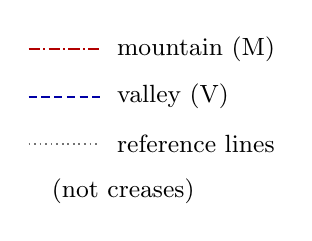
\begin{tikzpicture}[x=1cm,y=1cm,font=\small]
\draw[mtn] (0,2.2)--(0.9,2.2); \node[anchor=west] at (1,2.2) {mountain (M)};
\draw[val] (0,1.6)--(0.9,1.6); \node[anchor=west] at (1,1.6) {valley (V)};
\draw[refl] (0,1.0)--(0.9,1.0); \node[anchor=west] at (1,1.0) {reference lines};
\node[anchor=west,align=left] at (0,0.4) {\phantom{x}(not creases)};
\end{tikzpicture}
\caption{The running pattern, on the square $Q=[0,8]^2$. It has $84$ creases and $32$ interior vertices; every crease direction is a multiple of $\pi/32$. The dotted reference lines were used to place two creases and are not part of the pattern. The circled vertex $\vstar=(6,4)$ is where a crease appears to stop for no reason (Proposition~\ref{prop:vstar}).}
\label{fig:cp}
\end{figure}

\section{Introduction}

Fold a square flat, unfold it, and look at the creases. Each crease is a segment bent one of two ways, mountain or valley, and the labelled drawing is a \emph{crease pattern}. Designers publish crease patterns instead of step-by-step instructions because one picture records the whole design. It does not record the order of the folds. We ask how much of that order can be read back from the pattern alone:
\begin{itemize}
\item[(Q1)] Which creases must have been made by the same move?
\item[(Q2)] Which must have been made before which others?
\end{itemize}

The answer rests on one geometric fact (Lemma~\ref{lem:reflection}): when a fold passes through several layers, the creases it leaves in adjacent layers are mirror images across the crease that separates them. We apply this fact at one vertex at a time. At a vertex $v$, a \emph{local history} is a sequence of folds that produces exactly the creases at $v$, where each fold is made through one line in the paper as it is folded at that moment (Section~\ref{sec:local}). Theorem~\ref{thm:wedge} characterises local histories by a parity condition and a \emph{wedge condition}: two creases made by the same fold are related by the product of reflections in the earlier creases between them. This turns the history at a vertex into arithmetic on directions. A collision test (Lemma~\ref{lem:collision}) removes histories in which paper would pass through paper.

Two further ingredients complete the model. A fold that lands exactly on an existing crease erases it (Lemma~\ref{lem:cancel}); the erased segment leaves no trace in the pattern but is needed to explain it. We recover such \emph{cancelled segments} by requiring that they, too, have local histories wherever they meet the pattern (Section~\ref{sec:cancel}). And some moves fold several lines at once; we admit them at a cost, measured by the number of distinct fold lines they use (Section~\ref{sec:collapse}).

The global problem asks for one order of all creases, visible and cancelled, whose restriction to every vertex is a local history (Section~\ref{sec:global}). Its solutions are the \emph{resolutions} of the pattern. From the set of resolutions we read off the \emph{folds}, creases that are simultaneous in every resolution, which answer (Q1) from below, and the \emph{forced order}, which answers (Q2).

Everything here is a necessary condition for foldability by the moves we allow. We do not compute the order of layers in the folded stack, so a resolution is evidence for a folding sequence, not a certificate.

We work two small patterns by hand. The running pattern (Figure~\ref{fig:cp}) has $84$ creases. One of its vertices has no local history, and the theory repairs it with a single cancelled segment that it finds without being told where to look. The body pattern (Figure~\ref{fig:body}) has $15$ creases. It shows the collision test at work: a partition of the creases that satisfies every wedge condition is ruled out because paper would pass through paper. Section~\ref{sec:compute} describes the computation, Section~\ref{sec:dragon} applies it to a dragon with $278$ creases, and Section~\ref{sec:corpus} reports on $48$ patterns from a public collection. Section~\ref{sec:open} lists what remains open.

\section{Folding, reflection and cancellation}\label{sec:folding}

\begin{definition}
A \emph{crease pattern} on a polygon $Q$ is a finite set of closed segments in $Q$ (the \emph{creases}) that meet only at endpoints. The endpoints are \emph{vertices}; a vertex is \emph{interior} if it lies in the interior of $Q$. The creases divide $Q$ into convex polygons, the \emph{faces}.
\end{definition}

We work with the geometric shadow of folding: where each point of the paper goes, not how the layers are stacked.

\begin{definition}
A \emph{flat folded state} of a crease pattern is a continuous map $f\colon Q\to\R^2$ that is an isometry on each face and satisfies, for faces $F,F'$ sharing a crease $e$,
\begin{equation}\label{eq:fold}
f|_{F'} = f|_F\circ\rho_e,
\end{equation}
where $\rho_e$ is the reflection of the plane in the line through $e$.
\end{definition}

Equation~\eqref{eq:fold} says that the paper turns over at every crease.

\begin{definition}
A \emph{single-line move} along a line $\ell$ in the plane replaces $f$ by $f'=\rho_\ell\circ f$ on a union $M$ of faces (the \emph{moving} paper, after cutting faces along $f^{-1}(\ell)$ where necessary) and leaves $f$ unchanged elsewhere. Its new creases lie in $f^{-1}(\ell)$, exactly where moving and staying paper meet.
\end{definition}

\begin{lemma}[Reflection]\label{lem:reflection}
Let $F,F'$ be faces sharing a crease $e$, and suppose a move along $\ell$ makes new creases in both. Then inside $F\cup F'$ these creases are mirror images of each other in the line of $e$.
\end{lemma}

\begin{proof}
The new crease in $F'$ lies in $(f|_{F'})^{-1}(\ell)=(f|_F\circ\rho_e)^{-1}(\ell)=\rho_e\big((f|_F)^{-1}(\ell)\big)$.
\end{proof}

\begin{lemma}[Cancellation]\label{lem:cancel}
Let $e$ be a crease between faces $F,F'$ with $f(e)\subset\ell$. If a move along $\ell$ moves $F'$ but not $F$, then afterwards $e$ is no longer a crease.
\end{lemma}

\begin{proof}
Since $f|_F$ carries the line of $e$ onto $\ell$, $f|_F\circ\rho_e=\rho_\ell\circ f|_F$. Hence $f'|_{F'}=\rho_\ell\circ f|_{F'}=\rho_\ell\circ f|_F\circ\rho_e=f|_F\circ\rho_e\circ\rho_e=f'|_F$, so \eqref{eq:fold} no longer holds across $e$: the paper is flat there.
\end{proof}

A fold that lands exactly on an earlier crease therefore erases it, as does unfolding. We think of the erased segment as carrying two creases, one from each move, that cancel.

\begin{lemma}[Moving boundary]\label{lem:boundary}
Let $F,F'$ be faces sharing an edge $e$. If a move along $\ell$ moves $F'$ but not $F$, then $f(e)\subset\ell$.
\end{lemma}

\begin{proof}
A point $x\in e$ ends at $f(x)$ as a point of $F$ and at $\rho_\ell(f(x))$ as a point of $F'$. Continuity forces $\rho_\ell(f(x))=f(x)$.
\end{proof}

For the collision test we add one physical assumption: in a single-line move, each moving face turns rigidly through a half-turn about $\ell$, and paper cannot pass through paper.

\begin{lemma}[Collision]\label{lem:collision}
Let $F$ and $G$ be faces, neither creased by a single-line move along $\ell$, and let $\rho$ be a ray of $\ell$ such that $f(F)$ and $f(G)$ each contain, in their interiors, all points of $\rho$ close enough to its endpoint. Then $F$ and $G$ both move or both stay.
\end{lemma}

\begin{proof}
Suppose $F$ moves and $G$ stays. Near the endpoint of $\rho$, the images of $F$ and $G$ overlap on both sides of $\ell$, so in the stack one of them lies above the other there. In the half-turn of $F$ about $\ell$, the points of $F$ on one side of $\ell$ leave the plane upwards and those on the other side leave it downwards, whatever the sense of rotation. One of these two halves therefore sweeps through $G$ immediately (Figure~\ref{fig:collision}(b)).
\end{proof}

\section{Local histories}\label{sec:local}

\subsection{Directions and folding maps at a vertex}

Fix an interior vertex $v$. A crease at $v$ leaves $v$ along a ray, and we identify the ray with its direction $x\in\Dir$, measured counterclockwise from the positive $x$-axis. Two rays lie on one line exactly when their directions agree modulo $\pi$. Reflection in a line of direction $c$ acts on directions by
\[
\sigma_c(x)=2c-x,
\]
which depends only on $c$ modulo $\pi$. Every isometry $\varphi$ of the plane acts on directions as $x\mapsto \pm x+o$, and such maps respect congruence modulo $\pi$. If $\varphi$ is such a map and $x$ a direction, then
\begin{equation}\label{eq:conj}
\varphi\circ\sigma_x\circ\varphi^{-1}=\sigma_{\varphi(x)},
\end{equation}
as one checks in the two cases $\varphi(x)=x+o$ and $\varphi(x)=-x+o$.

A \emph{state} at $v$ is a finite set $S=\{s_1<\dots<s_m\}$ of rays, listed counterclockwise from some starting ray. Its \emph{sectors} are the open wedges $(s_j,s_{j+1})$, indices modulo $m$; if $S$ is empty there is one sector, the whole circle. The \emph{folding maps} of $S$ are
\[
\varphi_1=\mathrm{id},\qquad \varphi_{j+1}=\varphi_j\circ\sigma_{s_{j+1}},
\]
with $\varphi_j$ belonging to the sector that starts at $s_j$. They describe a flat folded state near $v$ exactly when going once around returns to the identity, $\varphi_m\circ\sigma_{s_1}=\mathrm{id}$; we then call $S$ \emph{flat}. This is Kawasaki's condition: $m$ is even and alternate angles sum to $\pi$~\cite{hull}. For a direction $x$ in the sector of $\varphi_j$, the \emph{image} of $x$ is $\varphi_j(x)$: the direction, in the folded state, of a ray from $v$ in direction $x$.

\subsection{Steps and histories}

By Lemma~\ref{lem:reflection}, a single-line move through the image of $v$ creases the paper near $v$ along rays whose images lie on the fold line, and by Lemma~\ref{lem:boundary} the paper switches between moving and staying exactly at those rays.

\begin{definition}\label{def:step}
Let $S$ be a flat state. A \emph{single-line step} from $S$ is a set $T$ of rays not in $S$ such that
\begin{itemize}
\item[(P)] $|T|$ is even;
\item[(L)] the images of the rays of $T$ under the folding maps of $S$ lie on one line;
\item[(C)] colouring the sectors of $S\cup T$ alternately moving and staying, switching at each ray of $T$, no two sectors of $S$ that contain no ray of $T$ and contain preimages of the same ray of that line receive different colours.
\end{itemize}
The new state is $S\cup T$.
\end{definition}

Condition (P) is the parity of the switches in Lemma~\ref{lem:boundary}, (L) is Lemma~\ref{lem:reflection}, and (C) is Lemma~\ref{lem:collision} applied to the sectors near $v$. A sector bounded by a ray of $T$ has one edge of its image on the fold line and cannot straddle it, which is why (C) concerns only uncut sectors of $S$.

\begin{definition}\label{def:history}
A \emph{local history} of a set $A$ of rays is a sequence of single-line steps $T_1,\dots,T_k$ from the empty state, with $T_1\cup\dots\cup T_k=A$. Equivalently, it is a weak order on $A$ whose classes, taken in order, are single-line steps. A weak order satisfying (P) and (L) at every step is a \emph{history up to collisions}.
\end{definition}

Section~\ref{sec:cancel} extends histories by steps that erase rays.

\begin{lemma}[Flat extension]\label{lem:flatext}
If $S$ is flat and $T$ satisfies (P) and (L) with respect to $S$, then $S\cup T$ is flat.
\end{lemma}

\begin{proof}
Let $\lambda$ be the line of the images in (L). Walk once around $v$, starting in a sector of $S\cup T$ that is contained in the first sector of $S$. Crossing a ray $s\in S$ in a sector of map $\varphi$ multiplies the map on the right by $\sigma_s$, as before. Crossing a ray $x\in T$ inside a sector of $S$ with map $\varphi$ multiplies on the right by $\sigma_x$, and $\varphi\sigma_x=\sigma_{\varphi(x)}\varphi=\sigma_\lambda\varphi$ by \eqref{eq:conj}. By induction the map after a crossing is $\sigma_\lambda^{c}\varphi$, where $\varphi$ is the corresponding map of $S$ and $c$ is the number of rays of $T$ crossed so far. Going all the way round gives $\sigma_\lambda^{|T|}\circ\mathrm{id}=\mathrm{id}$, because $|T|$ is even.
\end{proof}

\subsection{The wedge characterisation}

For rays $x\neq y$ and a state $S$, write $W_S(x,y)=(w_1,\dots,w_r)$ for the rays of $S$ strictly inside the counterclockwise wedge from $x$ to $y$, listed counterclockwise.

\begin{theorem}[Wedge characterisation]\label{thm:wedge}
A weak order on a set $A$ of rays at $v$, with classes $T_1<\dots<T_k$ and $S_j=T_1\cup\dots\cup T_{j-1}$, is a history up to collisions if and only if every $|T_j|$ is even and, for all $x,y\in T_j$,
\begin{equation}\label{eq:wedge}
y\equiv\sigma_{w_r}\circ\cdots\circ\sigma_{w_1}(x)\pmod\pi,\qquad (w_1,\dots,w_r)=W_{S_j}(x,y).
\end{equation}
The product has the closed form
\begin{equation}\label{eq:closed}
\sigma_{w_r}\circ\cdots\circ\sigma_{w_1}(x)=\begin{cases}2s-x & r\text{ odd},\\ x+2s & r\text{ even},\end{cases}\qquad s=w_r-w_{r-1}+\dots+(-1)^{r-1}w_1.
\end{equation}
\end{theorem}

\begin{proof}
Assume $S_j$ is flat, with folding maps $\varphi$. If $x$ lies in the sector with map $\varphi_x$ and $y$ in the sector with map $\varphi_y$, walking counterclockwise from $x$ to $y$ crosses exactly $w_1,\dots,w_r$, so $\varphi_y=\varphi_x\circ\sigma_{w_1}\circ\dots\circ\sigma_{w_r}$. The images of $x$ and $y$ lie on one line if and only if $\varphi_x(x)\equiv\varphi_x\sigma_{w_1}\cdots\sigma_{w_r}(y)\pmod\pi$. Since $\varphi_x$ and the $\sigma$'s respect congruence modulo $\pi$ and the $\sigma$'s are involutions, this holds if and only if~\eqref{eq:wedge} holds. Condition (L) for $T_j$ is~\eqref{eq:wedge} for all pairs in $T_j$, because lying on one common line is transitive.

Now argue by induction on $j$. The empty state is flat. If $S_j$ is flat and $T_j$ satisfies (P) and \eqref{eq:wedge}, it satisfies (P) and (L), so $S_{j+1}$ is flat by Lemma~\ref{lem:flatext}. Conversely, a history up to collisions has flat states throughout by the same lemma, and the computation above gives~\eqref{eq:wedge}. Finally, \eqref{eq:closed} follows by induction on $r$ from $\sigma_b\sigma_a(x)=x+2(b-a)$.
\end{proof}

\begin{figure}[t]
\centering
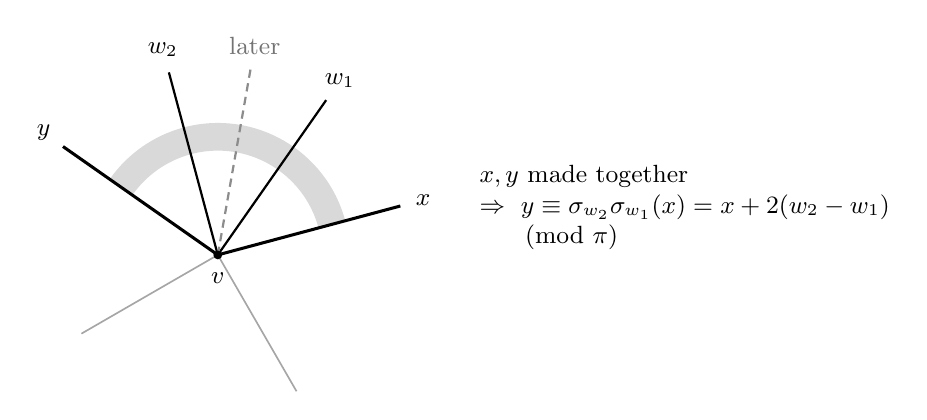
\begin{tikzpicture}[x=1cm,y=1cm,font=\small]
\draw[black!15,line width=10pt] (0,0) ++(15:1.5) arc (15:145:1.5);
\foreach \a/\n in {15/x,145/y} {\draw[line width=1.1pt] (0,0)--(\a:2.4); \node at (\a:2.7) {$\n$};}
\foreach \a/\n in {55/w_1,105/w_2} {\draw[line width=0.8pt] (0,0)--(\a:2.4); \node at (\a:2.7) {$\n$};}
\draw[line width=0.8pt,black!45,dash pattern=on 3pt off 2pt] (0,0)--(80:2.4); \node[black!55] at (80:2.7) {later};
\foreach \a in {210,300} \draw[line width=0.6pt,black!35] (0,0)--(\a:2.0);
\fill (0,0) circle (1.6pt); \node[anchor=north] at (0,-0.1) {$v$};
\node[anchor=west,align=left,font=\small] at (3.2,0.6) {$x,y$ made together\\ $\Rightarrow\ y\equiv \sigma_{w_2}\sigma_{w_1}(x)=x+2(w_2-w_1)$\\ \phantom{$\Rightarrow\ $}$\pmod\pi$};
\end{tikzpicture}
\caption{The wedge condition. Only the earlier creases strictly inside the counterclockwise wedge from $x$ to $y$ (shaded) enter; later creases and creases outside the wedge do not.}
\label{fig:wedge}
\end{figure}

The condition involves only the earlier creases in one wedge (Figure~\ref{fig:wedge}). Because $S_j$ is flat, the clockwise wedge gives the same condition.

\begin{corollary}\label{cor:wedge}
In a history up to collisions:
\begin{enumerate}
\item two rays made together with no earlier ray between them are collinear, $y=x+\pi$;
\item two rays made together with exactly one earlier ray $w$ between them satisfy $y\equiv\sigma_w(x)$: the second is the first reflected in $w$;
\item the first step is a single straight line through $v$;
\item a vertex with no two collinear rays has no local history.
\end{enumerate}
\end{corollary}

\begin{proof}
(1) and (2) are~\eqref{eq:closed} with $r=0$ and $r=1$. (3) is (1) with $S_1=\emptyset$, together with the fact that a line meets $v$ in at most two rays. (4) follows from (3).
\end{proof}

Items (1) and (2) are the two ways a chain of creases can continue through a vertex: straight on, or bent across one earlier crease. The theorem says that these are special cases of a single rule, in which a fold may bend across any number of earlier creases at once.

\begin{example}[A crossing]\label{ex:crossing}
In the running pattern, measure directions in units of $\pi/32$, so that directions are integers modulo $64$ and lines are integers modulo $32$. At $(6-2\sqrt2,6)\approx(3.172,6)$ the rays are $0,4,32,60$. By Corollary~\ref{cor:wedge}(3) the first step is $\{0,32\}$, the horizontal $A^+$. For $\{4,60\}$ the counterclockwise wedge from $60$ to $4$ contains the earlier ray $0$, and $60+4\equiv2\cdot0\pmod{32}$, so the second step is valid. Starting instead with $\{4,60\}$ fails, because these rays are not collinear. The vertex has exactly one local history: $A^+$, then the chain $P_1^+$ bending across it.
\end{example}

\begin{example}[Three folds at one point]\label{ex:three}
At $(4,8-4\sqrt2)\approx(4,2.343)$ the rays are $4,10,16,36,56,62$. The first step must be a line, and only $\{4,36\}$ is one; it belongs to the fold $P_1^-$. Next, $\{16,56\}$ has the single earlier ray $36$ in its wedge, and $16+56\equiv2\cdot36\pmod{32}$. The pair $\{10,62\}$ has $36$ in its wedge, and also $16$ and $56$ if $\{16,56\}$ came first. In the first case $10+62\equiv 2\cdot 36$; in the second $s=56-36+16=36$ and again $10+62\equiv2s$. So $C=\{16,56\}$ and $C'=\{10,62\}$ may come in either order after $P_1^-$. They cannot be made together, because their images under the fold along $P_1^-$ are the distinct lines $16$ and $10$. This vertex has two local histories.
\end{example}

\section{Collisions at a vertex}\label{sec:collisions}

Condition (C) is not implied by (P) and (L). The body pattern (Figure~\ref{fig:body}) shows this. Its directions are multiples of $\pi/4$; in this section we measure them in units of $\pi/4$, so directions are integers modulo $8$ and lines integers modulo $4$.

\begin{figure}[t]
\centering
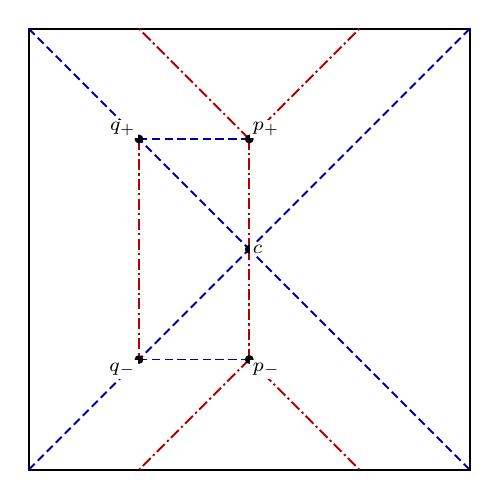
\begin{tikzpicture}[x=0.7cm,y=0.7cm]
\draw[sheet] (0,0) rectangle (8,8);
\draw[mtn] (4,4)--(4,6); \draw[mtn] (4,4)--(4,2); \draw[mtn] (2,6)--(2,2);
\draw[mtn] (4,2)--(2,0); \draw[mtn] (4,2)--(6,0); \draw[mtn] (4,6)--(2,8); \draw[mtn] (4,6)--(6,8);
\draw[val] (0,0)--(4,4); \draw[val] (0,8)--(4,4); \draw[val] (8,8)--(4,4); \draw[val] (8,0)--(4,4);
\draw[val] (4,2)--(2,2); \draw[val] (4,6)--(2,6);
\foreach \p/\n/\a in {(4,4)/c/west, (4,6)/p_+/south west, (4,2)/p_-/north west, (2,6)/q_+/south east, (2,2)/q_-/north east}
  {\fill \p circle (1.6pt); \node[font=\scriptsize,anchor=\a,fill=white,inner sep=1pt] at \p {$\n$};}
\end{tikzpicture}
\caption{The body pattern on $Q=[0,8]^2$, drawn with the conventions of Figure~\ref{fig:cp}. Its interior vertices are the centre $c$, the points $p_\pm$ on the central vertical, and the corners $q_\pm$ of the rectangle.}
\label{fig:body}
\end{figure}

\begin{proposition}\label{prop:c}
The centre $c=(4,4)$ of the body pattern, with rays $1,2,3,5,6,7$, has exactly two local histories: the vertical $X=\{2,6\}$, then $V^+=\{1,3\}$ and $V^-=\{5,7\}$ in either order. Two further weak orders are histories up to collisions: the diagonals $D_1=\{1,5\}$ and $D_2=\{3,7\}$ in either order, then $X$. Condition (C) rejects both.
\end{proposition}

\begin{proof}
By Corollary~\ref{cor:wedge}(3) the first step is one of the three lines $X$, $D_1$, $D_2$.

After $X$, a diagonal cannot be made: the wedge from $1$ to $5$ contains the earlier ray $2$, and $1+5\not\equiv2\cdot2\pmod4$, and similarly for $\{3,7\}$, whose wedge contains $6$. The pair $\{1,3\}$ has the earlier ray $2$ in its wedge, and $1+3\equiv2\cdot2$, so it is valid; similarly $\{5,7\}$ with $6$. The two V's cannot be made together, because their images are the distinct lines $3$ and $1$. Condition (C) holds for these steps: the moving paper lies on one side of the fold line, as when an ordinary flap is folded.

After $D_1$, the line $D_2$ is valid, since its wedge from $3$ to $7$ contains the single earlier ray $5$ and $3+7\equiv2\cdot5\pmod 4$. The same holds after $D_2$. Then $X$ has the earlier rays $3,5$ in its wedge, with $s=5-3$, and $6-2\equiv 2s\pmod4$. So both orders pass (P) and (L).

For (C), fold $X$ after both diagonals. The four sectors $E,N,W,S$ between the diagonals are stacked on one quarter-turn wedge, and both halves of the vertical land on its bisector, which is therefore the fold line (Figure~\ref{fig:collision}(a)). The sectors $E$ and $W$ are not cut by the new rays, yet both contain preimages of the same ray of the fold line. The moving paper is one whole side of the vertical, so exactly one of $E$, $W$ moves. Condition (C) fails, and Lemma~\ref{lem:collision} shows why (Figure~\ref{fig:collision}(b)).
\end{proof}

\begin{figure}[t]
\centering
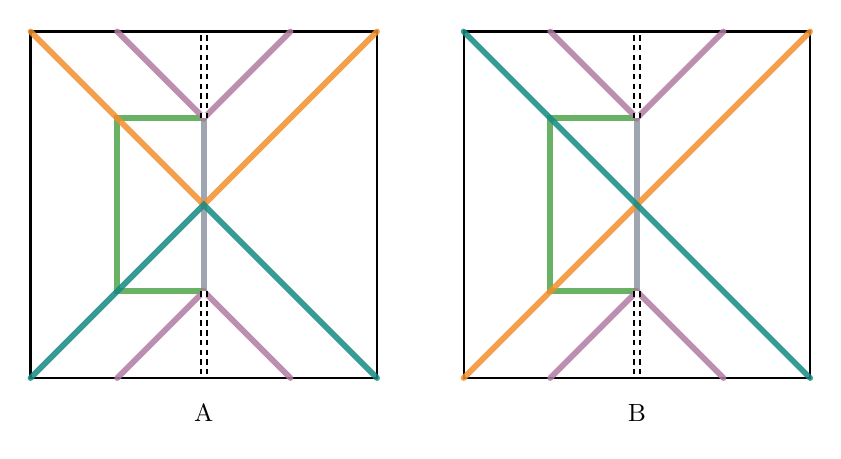
\begin{tikzpicture}[x=0.55cm,y=0.55cm]
\begin{scope}
\draw[sheet] (0,0) rectangle (8,8);
\draw[ch,cA] (4,2)--(4,6);
\draw[ch,cF] (4,6)--(2,6)--(2,2)--(4,2);
\draw[ch,cP2] (2,8)--(4,6)--(6,8); \draw[ch,cP2] (2,0)--(4,2)--(6,0);
\draw[ch,cP1] (0,8)--(4,4)--(8,8);
\draw[ch,cC] (0,0)--(4,4)--(8,0);
\draw[virt] (4,6)--(4,8); \draw[virt] (4,2)--(4,0);
\node[font=\small] at (4,-0.8) {A};
\end{scope}
\begin{scope}[xshift=5.5cm]
\draw[sheet] (0,0) rectangle (8,8);
\draw[ch,cA] (4,2)--(4,6);
\draw[ch,cF] (4,6)--(2,6)--(2,2)--(4,2);
\draw[ch,cP2] (2,8)--(4,6)--(6,8); \draw[ch,cP2] (2,0)--(4,2)--(6,0);
\draw[ch,cP1] (0,0)--(8,8);
\draw[ch,cC] (0,8)--(8,0);
\draw[virt] (4,6)--(4,8); \draw[virt] (4,2)--(4,0);
\node[font=\small] at (4,-0.8) {B};
\end{scope}
\end{tikzpicture}
\caption{Two partitions of the creases of the body pattern into folds, with the cancelled segments above $p_+$ and below $p_-$ (double dotted). Grey: the vertical $X$; green: the rectangle $R$; mauve: the small V's $U$ and $L$; orange and teal: the big V's $V^+$ and $V^-$ (left) or the diagonals $D_1$ and $D_2$ (right). Both satisfy the wedge conditions at $c$; only the left one survives the collision condition (Proposition~\ref{prop:c}).}
\label{fig:bodyres}
\end{figure}
\begin{figure}[t]
\centering
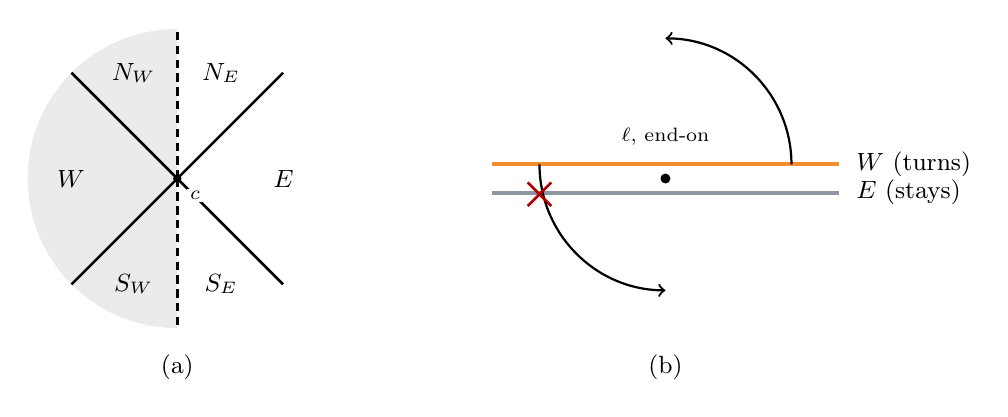
\begin{tikzpicture}[x=1cm,y=1cm,font=\small]
\begin{scope}
\fill[black!8] (0,0) -- (90:1.9) arc (90:270:1.9) -- cycle;
\foreach \a in {45,135,225,315} \draw[line width=0.9pt] (0,0)--(\a:1.9);
\foreach \a in {90,270} \draw[line width=0.9pt,dash pattern=on 3pt off 2pt] (0,0)--(\a:1.9);
\node at (0:1.35) {$E$}; \node at (180:1.35) {$W$};
\node at (67.5:1.45) {$N_E$}; \node at (112.5:1.45) {$N_W$};
\node at (247.5:1.45) {$S_W$}; \node at (292.5:1.45) {$S_E$};
\fill (0,0) circle (1.5pt); \node[anchor=north west,font=\scriptsize,fill=white,inner sep=1pt] at (0.12,-0.12) {$c$};
\node at (0,-2.4) {(a)};
\end{scope}
\begin{scope}[xshift=6.2cm]
\draw[line width=1.4pt,cP1] (-2.2,0.18)--(2.2,0.18); \node[anchor=west] at (2.3,0.18) {$W$ (turns)};
\draw[line width=1.4pt,cA] (-2.2,-0.18)--(2.2,-0.18); \node[anchor=west] at (2.3,-0.18) {$E$ (stays)};
\fill (0,0) circle (1.8pt); \node[anchor=south,font=\scriptsize] at (0,0.3) {$\ell$, end-on};
\draw[->,line width=0.8pt] (-1.6,0.18) arc (180:270:1.6);
\draw[->,line width=0.8pt] (1.6,0.18) arc (0:90:1.6);
\draw[red!70!black,line width=1pt] (-1.75,-0.35)--(-1.45,-0.05) (-1.75,-0.05)--(-1.45,-0.35);
\node at (0,-2.4) {(b)};
\end{scope}
\end{tikzpicture}
\caption{(a) The state at $c$ in partition B just before the vertical (dashed) is folded: the diagonals divide the paper into sectors $E,N,W,S$, and the vertical cuts $N$ and $S$ in half. The moving paper is one whole side of the vertical, for instance the shaded one. (b) Cross-section through the stack, looking along the fold line $\ell$. The sector $W$ straddles $\ell$ and turns over about it while $E$, which straddles the same ray, stays. The two halves of $W$ leave the plane in opposite directions, so one of them passes through $E$ (cross).}
\label{fig:collision}
\end{figure}

The partition into $X$, $D_1$, $D_2$ is therefore excluded at $c$ itself (Figure~\ref{fig:bodyres}, right), and no global reasoning is needed to exclude it. Folding all three lines at once would produce it, but that is a move through several lines, which Section~\ref{sec:collapse} treats separately.

\section{Cancellation}\label{sec:cancel}

\subsection{Erasing steps}

By Lemma~\ref{lem:cancel}, a move can erase an existing crease, and the erased crease does not appear in the pattern. At a vertex this gives a second kind of step. A \emph{hidden ray} is a ray created by one step and erased by a later one; it carries two creases, the \emph{first} and the \emph{cancelling} crease. A step may now also contain rays of the current state that are hidden: such rays are switch rays for (P), (L) and (C), and they leave the state. Visible rays are never erased. A \emph{local history with cancellations} of a set $A$ of visible rays is a sequence of such steps from the empty state that ends in the state $A$. Theorem~\ref{thm:wedge} applies to each step unchanged, with $S_j$ the current state. The following vertex needs three hidden rays.

\begin{figure}[t]
\centering
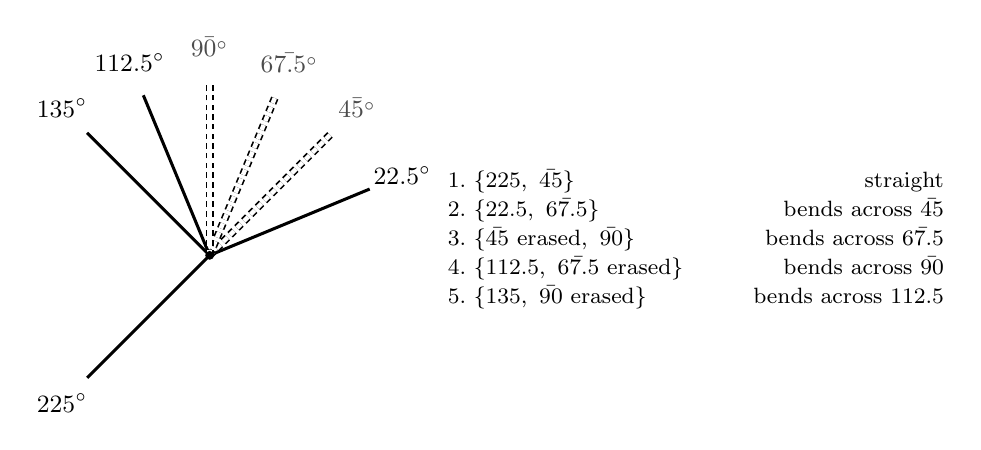
\begin{tikzpicture}[x=1cm,y=1cm,font=\small]
\foreach \a/\n in {22.5/22.5^\circ,112.5/112.5^\circ,135/135^\circ,225/225^\circ} {\draw[line width=1.1pt] (0,0)--(\a:2.2); \node at (\a:2.65) {$\n$};}
\foreach \a/\n in {45/45^\circ,67.5/67.5^\circ,90/90^\circ} {\draw[virt] (0,0)--(\a:2.2); \node[black!70] at (\a:2.65) {$\hid{\n}$};}
\fill (0,0) circle (1.6pt);
\node[anchor=west,align=left,font=\footnotesize,text width=6.3cm] at (2.9,0.2) {%
1.\ $\{225,\ \hid{45}\}$ \hfill straight\\[1pt]
2.\ $\{22.5,\ \hid{67.5}\}$ \hfill bends across $\hid{45}$\\[1pt]
3.\ $\{\hid{45}\ \text{erased},\ \hid{90}\}$ \hfill bends across $\hid{67.5}$\\[1pt]
4.\ $\{112.5,\ \hid{67.5}\ \text{erased}\}$ \hfill bends across $\hid{90}$\\[1pt]
5.\ $\{135,\ \hid{90}\ \text{erased}\}$ \hfill bends across $112.5$};
\end{tikzpicture}
\caption{A staircase of cancellations at a vertex of Komatsu's Horned Owl. Solid: the four visible creases. Double dotted: three hidden rays, each created by one step and erased by a later one. Each step bends across the ray made just before it.}
\label{fig:stair}
\end{figure}

\begin{example}[A staircase]\label{ex:stair}
Take the vertex of Komatsu's Horned Owl with visible rays at $22.5^\circ$, $112.5^\circ$, $135^\circ$ and $225^\circ$ (Figure~\ref{fig:stair}). No two are collinear, so by Corollary~\ref{cor:wedge}(4) there is no history without cancellations. The history in the figure uses three hidden rays. Step~1 is a line. In each later step the counterclockwise wedge between the two switch rays contains exactly one ray of the current state, the one made just before, and the step is its reflection: $22.5+67.5=2\cdot45$, $45+90=2\cdot67.5$, $67.5+112.5=2\cdot90$, $90+135=2\cdot112.5$. Each step after the second erases the hidden ray made two steps earlier, and the state ends with the four visible rays. An exhaustive search over hidden rays at multiples of $22.5^\circ$ finds no history with fewer than three.
\end{example}

\subsection{The history pattern}

A hidden ray at $v$ is the end of a cancelled segment running across the sheet, and that segment must be explained wherever it meets the pattern.

\begin{definition}\label{def:historypattern}
A \emph{history pattern} for a crease pattern $\mathcal P$ consists of $\mathcal P$ together with finitely many \emph{cancelled segments}, each carrying a first and a cancelling crease, and an order (a weak order) on all creases, such that:
\begin{itemize}
\item every vertex of the combined arrangement has a local history with cancellations consistent with the order, and erases no visible crease;
\item every point where cancelled creases meet, bend or end is a vertex of the combined arrangement.
\end{itemize}
\end{definition}

The vertices of the combined arrangement include those of $\mathcal P$, the points where a cancelled segment crosses a crease, and its bends and ends. The next lemma settles the crossings.

\begin{lemma}[Crossing]\label{lem:crossing}
Let a cancelled segment with creases $h_1$ (first) and $h_2$ (cancelling) cross a crease $z$ at a point $q$ interior to both. Then the history at $q$ is one of the following:
\begin{enumerate}
\item $z$ is later than $h_2$, and the segment passes straight through $q$;
\item $z$ is earlier than $h_1$, and the segment bends at $q$, continuing as its mirror image in $z$;
\item $z$ is perpendicular to the segment, which passes straight through $q$, in any order.
\end{enumerate}
\end{lemma}

\begin{proof}
At $q$ the visible rays are the two halves of $z$, made in one step, and the hidden rays are an incoming ray $a$ and an outgoing ray $b$, each carrying $h_1$ and $h_2$. The steps are $\{a,b\}$ for $h_1$, then $\{a,b\}$ for $h_2$, erasing them, and the step $z$ somewhere among them.
\begin{itemize}
\item If $z$ comes first, the wedge from $a$ to $b$ contains one half of $z$, so $b\equiv\sigma_z(a)$ by Corollary~\ref{cor:wedge}(2).
\item If $z$ comes last, the paper at $q$ is flat when the hidden steps are made, and $b=a+\pi$.
\item If $z$ comes between them, the step $\{a,b\}$ for $h_1$ is the first step at $q$, so $b=a+\pi$. When $z$ is made, the wedge from one half of $z$ to the other contains exactly one of $a,b$, and \eqref{eq:wedge} gives $2z+\pi\equiv2a\pmod\pi$, that is $2z\equiv 2a\pmod\pi$. Since $z\not\equiv a\pmod\pi$, this means $z\perp a$.
\end{itemize}
In every case with a straight segment and $z$ perpendicular, all three orders pass.
\end{proof}

So a cancelled segment can be traced from either end: through a later crease it continues straight, at an earlier crease it reflects, and a perpendicular crease leaves it unchanged. A cancelled segment ends at the boundary, or at a vertex of $\mathcal P$ whose local history contains the arriving hidden ray.

\begin{proposition}\label{prop:vstar}
The vertex $\vstar=(6,4)$ of the running pattern, with rays $12,32,40,52$ in units of $\pi/32$, has no local history without cancellations. With one hidden ray at $\vstar$, there is exactly one: the hidden ray $\hid0$ (direction $0$), and the history
\[
\{32,\hid0\}\ \to\ \{12,52\}\ \to\ \{40,\hid0\text{ erased}\}.
\]
The cancelled segment runs from $\vstar$ to the boundary point $(8,4)$ without meeting another crease.
\end{proposition}

\begin{proof}
No two rays at $\vstar$ are collinear, so Corollary~\ref{cor:wedge}(4) excludes histories without cancellations. Enumerating the hidden directions in units of $\pi/32$ and the step sequences (the computation of Section~\ref{sec:compute}) leaves only the history shown. Its steps can be checked by hand.
\begin{itemize}
\item The first step is a line, $32$ and $0$.
\item The wedge from $12$ to $52$ contains the earlier ray $32$ and the later ray $40$; $12+52=64\equiv2\cdot32\pmod{32}$.
\item The wedge from $40$ to $\hid0$ contains only $52$; $40+64=104\equiv2\cdot52\pmod{32}$.
\end{itemize}
The ray from $(6,4)$ in direction $0$ reaches $(8,4)$ without meeting a crease.
\end{proof}

Read as folding history: the horizontal crease $A^0$ along $y=4$ once ran to the edge, the fold $I$ was made across it, and later the fold $F$ landed exactly on its right-hand part and erased it. The vertex was found because it has no history; the direction of the erased segment was forced.

\section{Resolutions, folds and the forced order}\label{sec:global}

\begin{definition}\label{def:resolution}
A \emph{resolution} of a crease pattern $\mathcal P$ is a history pattern for $\mathcal P$ (Definition~\ref{def:historypattern}). Its \emph{geometry} is its set of cancelled segments. Its \emph{cost} is the pair $(\kappa,\eta)$, compared lexicographically: $\kappa$ is the total cost of the multi-line moves of Section~\ref{sec:collapse} ($0$ if there are none), and $\eta$ is the number of hidden rays at vertices of $\mathcal P$. A resolution is \emph{minimal} if no resolution has smaller cost.
\end{definition}

Counting hidden rays at visible vertices counts a cancelled segment once for each end that lies at a vertex of $\mathcal P$. This rewards segments that join two vertices that each need one.

Fix a geometry. Every order that makes it a resolution determines, at each vertex, which creases are made in the same step. We read the answers to (Q1) and (Q2) off what all these orders have in common.

\begin{definition}\label{def:folds}
Two creases at a common vertex are \emph{forced together} if they are made in the same step in every resolution with the given geometry. The \emph{folds} are the connected components of the relation ``forced together''. A fold $K$ is \emph{forced before} a fold $K'$ if every crease of $K$ is earlier than every crease of $K'$ in every such resolution.
\end{definition}

\begin{proposition}\label{prop:moves}
In any resolution with the given geometry, the creases made by one move form a union of folds, and the forced order is a partial order on the folds.
\end{proposition}

\begin{proof}
Creases forced together share a time in every resolution, and so do all creases of a fold, by connectedness. A move is a set of creases sharing a time, so it is a union of folds. The forced order is irreflexive and transitive, because it is the intersection of the strict orders that the resolutions induce on folds.
\end{proof}

Folds answer (Q1) from below. A fold is made by one move, but one move may make several folds, for instance the two mirror-image creases of a fold through a stack. Merging folds into moves requires global geometry, which we discuss in Section~\ref{sec:open}.

\begin{theorem}\label{thm:running}
The running pattern has no resolution without cancelled segments. It has exactly one minimal resolution, whose geometry is the single cancelled segment from $\vstar$ to $(8,4)$. In it:
\begin{enumerate}
\item there are $15$ folds (Figure~\ref{fig:folds1}): the horizontals $A^+,A^0,A^-$ along $y=6,4,2$; three pairs $P_1^\pm,P_2^\pm,P_3^\pm$ of mirror-image folds at the right end of the sheet; $I$ and $F$, which meet at $\vstar$; the folds $C,C'$ near $x=4$; and $E,E'$ near $x=1.3$;
\item the forced order has $30$ relations, its Hasse diagram has the $19$ edges of Figure~\ref{fig:hasse1}, and it has $172{,}768{,}020$ linear extensions;
\item the three horizontals are minimal, and $A^0$ is forced before $I$, which is forced before $F$;
\item $E$ is incomparable with every other fold.
\end{enumerate}
\end{theorem}

\begin{proof}
By Corollary~\ref{cor:wedge}(4) and Proposition~\ref{prop:vstar}, $\vstar$ needs a hidden ray, and with one hidden ray its history is unique. The other $31$ interior vertices have local histories without cancellations, listed in Appendix~\ref{app:table}. The cancelled segment from $\vstar$ meets no crease, so it adds no vertex, and the minimal cost is one hidden ray. The folds and the forced order are computed as in Section~\ref{sec:analysis}, and the count of linear extensions by dynamic programming over subsets of folds.
\end{proof}

\begin{figure}[t]
\centering
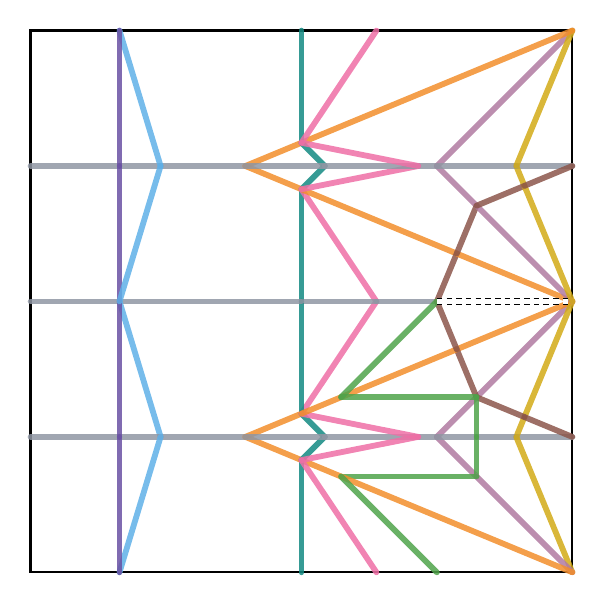
\begin{tikzpicture}[x=0.86cm,y=0.86cm]
\draw[sheet] (0,0) rectangle (8,8);
\draw[ch,cA] (8,6) -- (7.172,6);
\draw[ch,cA] (8,2) -- (7.172,2);
\draw[ch,cP2] (6,2) -- (6.586,1.414);
\draw[ch,cA] (6,2) -- (5.725,2);
\draw[ch,cP2] (8,4) -- (6.586,2.586);
\draw[ch,cP2] (6,6) -- (6.586,5.414);
\draw[ch,cA] (6,6) -- (5.725,6);
\draw[ch,cP2] (8,8) -- (6,6);
\draw[ch,cP1] (3.172,6) -- (4,6.343);
\draw[ch,cA] (3.172,6) -- (1.92,6);
\draw[ch,cP1] (3.172,2) -- (4,1.657);
\draw[ch,cA] (3.172,2) -- (1.92,2);
\draw[ch,cP1] (3.172,6) -- (4,5.657);
\draw[ch,cP3] (7.172,2) -- (7.293,2.293);
\draw[ch,cA] (7.172,2) -- (6.586,2);
\draw[ch,cP3] (8,0) -- (7.172,2);
\draw[ch,cP3] (7.172,6) -- (7.293,5.707);
\draw[ch,cA] (7.172,6) -- (6,6);
\draw[ch,cP3] (7.172,6) -- (8,8);
\draw[ch,cP1] (4,6.343) -- (8,8);
\draw[ch,cP1] (4,1.657) -- (4.586,1.414);
\draw[ch,cP1] (4,2.343) -- (3.172,2);
\draw[ch,cC] (4,5.657) -- (4.343,6);
\draw[ch,cC] (4.343,6) -- (4,6.343);
\draw[ch,cC] (4,6.343) -- (4,8);
\draw[ch,cC] (4,5.657) -- (4,4);
\draw[ch,cC] (4,2.343) -- (4.343,2);
\draw[ch,cC] (4.343,2) -- (4,1.657);
\draw[ch,cC] (4,1.657) -- (4,0);
\draw[ch,cA] (3.172,2) -- (4.343,2);
\draw[ch,cA] (3.172,6) -- (4.343,6);
\draw[ch,cCp] (4,2.343) -- (5.107,4);
\draw[ch,cCp] (4,5.657) -- (5.107,4);
\draw[ch,cA] (5.107,4) -- (4,4);
\draw[ch,cC] (4,4) -- (4,2.343);
\draw[ch,cP1] (8,4) -- (6.293,3.293);
\draw[ch,cP1] (4,5.657) -- (6.293,4.707);
\draw[ch,cA] (4,4) -- (1.313,4);
\draw[ch,cCp] (5.725,6) -- (4,5.657);
\draw[ch,cA] (5.725,6) -- (4.343,6);
\draw[ch,cCp] (4,6.343) -- (5.725,6);
\draw[ch,cCp] (5.107,8) -- (4,6.343);
\draw[ch,cA] (5.725,2) -- (4.343,2);
\draw[ch,cCp] (4,2.343) -- (5.725,2);
\draw[ch,cCp] (5.725,2) -- (4,1.657);
\draw[ch,cCp] (5.107,0) -- (4,1.657);
\draw[ch,cEp] (1.313,4) -- (1.92,2);
\draw[ch,cA] (1.92,2) -- (1.313,2);
\draw[ch,cA] (1.313,4) -- (0,4);
\draw[ch,cEp] (1.92,2) -- (1.313,0);
\draw[ch,cA] (1.92,6) -- (1.313,6);
\draw[ch,cEp] (1.92,6) -- (1.313,8);
\draw[ch,cA] (1.313,2) -- (0,2);
\draw[ch,cA] (1.313,6) -- (0,6);
\draw[ch,cE] (1.313,4) -- (1.313,6);
\draw[ch,cE] (1.313,6) -- (1.313,8);
\draw[ch,cE] (1.313,4) -- (1.313,2);
\draw[ch,cE] (1.313,2) -- (1.313,0);
\draw[ch,cP3] (7.293,2.293) -- (8,4);
\draw[ch,cI] (8,2) -- (7.293,2.293);
\draw[ch,cI] (7.293,2.293) -- (6.586,2.586);
\draw[ch,cP2] (6.586,2.586) -- (6,2);
\draw[ch,cI] (6.586,2.586) -- (6.293,3.293);
\draw[ch,cP1] (6.293,3.293) -- (4.586,2.586);
\draw[ch,cI] (6.293,3.293) -- (6,4);
\draw[ch,cA] (6,4) -- (5.107,4);
\draw[ch,cI] (6,4) -- (6.293,4.707);
\draw[ch,cP1] (6.293,4.707) -- (8,4);
\draw[ch,cI] (6.293,4.707) -- (6.586,5.414);
\draw[ch,cP2] (6.586,5.414) -- (8,4);
\draw[ch,cI] (6.586,5.414) -- (7.293,5.707);
\draw[ch,cP3] (7.293,5.707) -- (8,4);
\draw[ch,cI] (7.293,5.707) -- (8,6);
\draw[ch,cP1] (4.586,2.586) -- (4,2.343);
\draw[ch,cF] (6,4) -- (4.586,2.586);
\draw[ch,cF] (4.586,2.586) -- (6.586,2.586);
\draw[ch,cA] (6.586,2) -- (6,2);
\draw[ch,cF] (6.586,2.586) -- (6.586,2);
\draw[ch,cF] (6.586,2) -- (6.586,1.414);
\draw[ch,cP2] (6.586,1.414) -- (8,0);
\draw[ch,cF] (6.586,1.414) -- (4.586,1.414);
\draw[ch,cP1] (4.586,1.414) -- (8,0);
\draw[ch,cF] (4.586,1.414) -- (6,0);
\draw[ch,cEp] (1.313,4) -- (1.92,6);
\draw[virt] (6,4) -- (8,4);
\end{tikzpicture}
\hspace{0.8em}
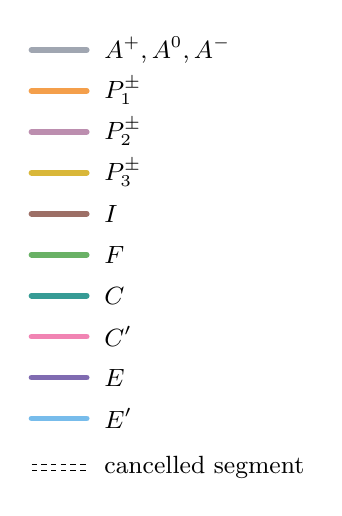
\begin{tikzpicture}[x=1cm,y=0.52cm,font=\small]
\foreach \c/\n [count=\i] in {cA/{$A^{+},A^{0},A^{-}$},cP1/{$P_1^{\pm}$},cP2/{$P_2^{\pm}$},cP3/{$P_3^{\pm}$},cI/{$I$},cF/{$F$},cC/{$C$},cCp/{$C'$},cE/{$E$},cEp/{$E'$}}{
  \draw[ch,\c] (0,-\i)--(0.7,-\i); \node[anchor=west] at (0.8,-\i) {\n};}
\draw[virt] (0,-11.2)--(0.7,-11.2); \node[anchor=west] at (0.8,-11.2) {cancelled segment};
\end{tikzpicture}
\caption{The $15$ folds of the running pattern in its unique minimal resolution. A superscript $+$ marks the upper member of a pair of folds that are mirror images in the line $y=4$. The double dotted segment from $\vstar=(6,4)$ to $(8,4)$ is the cancelled segment: its first crease belongs to $A^0$, its second to $F$.}
\label{fig:folds1}
\end{figure}
\begin{figure}[t]
\centering
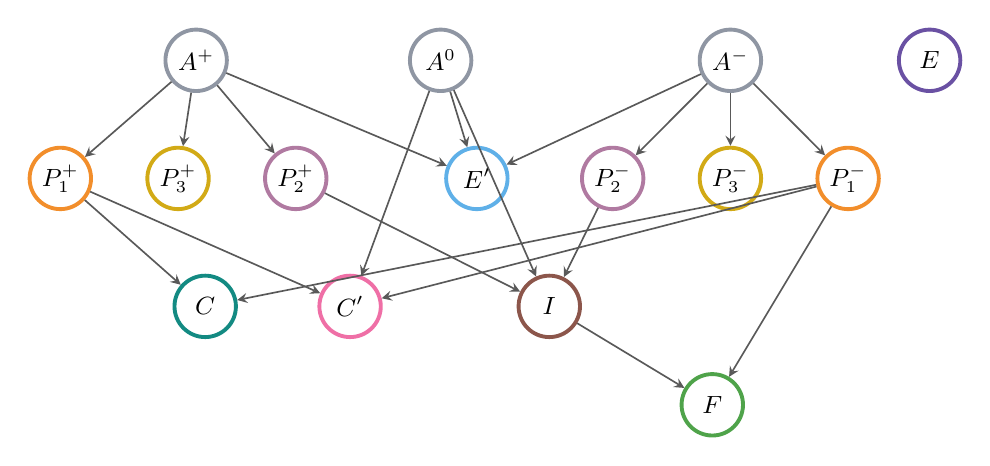
\begin{tikzpicture}[x=1.15cm,y=1.25cm,font=\small,>=stealth,
  nd/.style={circle,inner sep=1.2pt,minimum size=0.78cm,line width=1.4pt,fill=white}]
\node[nd,draw=cA] (Ap) at (1.5,3) {$A^{+}$};
\node[nd,draw=cA] (A0) at (4.2,3) {$A^{0}$};
\node[nd,draw=cA] (Am) at (7.4,3) {$A^{-}$};
\node[nd,draw=cE] (E) at (9.6,3) {$E$};
\node[nd,draw=cP1] (P1p) at (0,1.8) {$P_1^{+}$};
\node[nd,draw=cP3] (P3p) at (1.3,1.8) {$P_3^{+}$};
\node[nd,draw=cP2] (P2p) at (2.6,1.8) {$P_2^{+}$};
\node[nd,draw=cEp] (Ep) at (4.6,1.8) {$E'$};
\node[nd,draw=cP2] (P2m) at (6.1,1.8) {$P_2^{-}$};
\node[nd,draw=cP3] (P3m) at (7.4,1.8) {$P_3^{-}$};
\node[nd,draw=cP1] (P1m) at (8.7,1.8) {$P_1^{-}$};
\node[nd,draw=cC] (C) at (1.6,0.5) {$C$};
\node[nd,draw=cCp] (Cp) at (3.2,0.5) {$C'$};
\node[nd,draw=cI] (I) at (5.4,0.5) {$I$};
\node[nd,draw=cF] (F) at (7.2,-0.5) {$F$};
\foreach \a/\b in {Ap/P2p,Ap/P1p,Ap/P3p,Ap/Ep,Am/P2m,Am/P1m,Am/P3m,Am/Ep,A0/Cp,A0/Ep,A0/I,P2m/I,P2p/I,P1p/C,P1p/Cp,P1m/C,P1m/Cp,P1m/F,I/F}
  \draw[->,line width=0.6pt,black!65] (\a) -- (\b);
\end{tikzpicture}
\caption{Hasse diagram of the forced order on the folds of the running pattern. An arrow $K\to K'$ means that $K$ is made before $K'$ in every resolution with this geometry.}
\label{fig:hasse1}
\end{figure}

Item~4 has a simple cause. The fold $E$ is the vertical line $x=8\sqrt2-10\approx1.313$, and it meets other creases only at right angles. At a vertex where two perpendicular lines cross, either order passes Theorem~\ref{thm:wedge}, because the wedge of the second line contains one earlier ray $w$ with $x+(x+\pi)\equiv2w\pmod\pi$ exactly when $w\perp x$. Right-angle crossings carry no ordering information, and they account for much of the large number of linear extensions.

\begin{theorem}\label{thm:body}
The body pattern has exactly one minimal resolution. Its geometry is two cancelled segments, continuing the central vertical from $p_+$ to $(4,8)$ and from $p_-$ to $(4,0)$. It has $6$ folds, partitioned as on the left of Figure~\ref{fig:bodyres}, and the forced order is generated by
\[
X\prec U,\,L,\,V^+,\,V^-\prec R,
\]
with $9$ relations, $8$ Hasse edges and $24$ linear extensions.
\end{theorem}

\begin{proof}
The vertices $p_\pm$ have no collinear rays, so each needs a hidden ray. Locally, two directions work at $p_+$: the vertical continuation, and a diagonal into the sheet; the same holds at $p_-$ by symmetry. Only the vertical continuations extend to a resolution. At $c$ the histories are those of Proposition~\ref{prop:c}. At $p_+$ the history is: the vertical $X$ with the first hidden crease, then the small V $U$ bending across it, then $R$ bending across $U$ and erasing the hidden ray; $p_-$ is symmetric. The order follows.
\end{proof}

In folding terms: fold the sheet in half along $X$, make the big and small V's through both layers in any order, then make the rectangle fold $R$, which erases the two ends of $X$.

\section{Moves through several lines}\label{sec:collapse}

Some moves fold several lines at once: squash folds, petal folds, sinks and twists. In the plane, such a move replaces $f$ by $g_i\circ f$ on regions $M_i$, for isometries $g_i$.

\begin{lemma}[Boundaries of a move]\label{lem:multiboundary}
Let a move replace $f$ by $g\circ f$ on a face $F$ and by $g'\circ f$ on an adjacent face $F'$, across their common edge $e$.
\begin{enumerate}
\item If $e$ becomes a new crease, then $g^{-1}g'$ is the reflection in a line containing $f(e)$.
\item If $e$ was a crease and remains one, then $g=g'$.
\end{enumerate}
\end{lemma}

\begin{proof}
(1) Before the move $f|_{F'}=f|_F$, and afterwards \eqref{eq:fold} requires $g'f|_{F'}=gf|_F\circ\rho_e$. Hence $g^{-1}g'=f|_F\,\rho_e\,f|_F^{-1}$, the reflection in the line $f(e)$. (2) Before the move $f|_{F'}=f|_F\rho_e$; afterwards $g'f|_{F'}=gf|_F\rho_e$. Hence $g'=g$.
\end{proof}

At a vertex, then, the new creases of a move map onto a set of lines through the image of $v$, one for each relative isometry $g^{-1}g'$ that occurs. We call the number of these lines the \emph{width} of the move. A single-line move has width $1$, and a move of width $w$ costs $w-1$. A \emph{collapse step} at $v$ is any set $T$ of new rays such that $S\cup T$ is flat; its width is the number of distinct lines among the images of $T$. Allowing collapse steps makes every flat vertex resolvable in one step, which is why they carry a cost.

\begin{figure}[t]
\centering
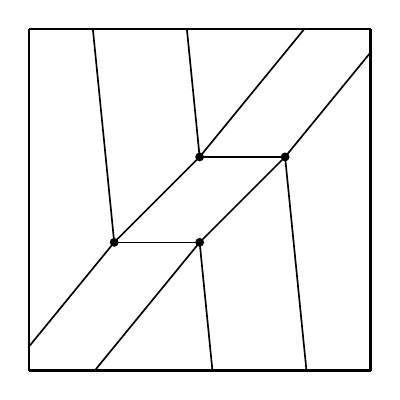
\begin{tikzpicture}[x=0.62cm,y=0.62cm]
\draw[sheet] (3.762,0.000) -- (1.352,0.000);
\draw[sheet] (0.000,0.486) -- (0.000,7.000);
\draw[sheet] (7.000,7.000) -- (7.000,6.514);
\draw[sheet] (1.312,7.000) -- (3.238,7.000);
\draw[sheet] (1.352,0.000) -- (0.000,0.000);
\draw[sheet] (0.000,7.000) -- (1.312,7.000);
\draw[sheet] (5.648,7.000) -- (3.238,7.000);
\draw[sheet] (7.000,6.514) -- (7.000,0.000);
\draw[sheet] (3.762,0.000) -- (5.688,0.000);
\draw[sheet] (0.000,0.486) -- (0.000,0.000);
\draw[sheet] (5.648,7.000) -- (7.000,7.000);
\draw[sheet] (7.000,0.000) -- (5.688,0.000);
\draw[crease] (0.000,0.486) -- (1.750,2.625);
\draw[crease] (3.500,4.375) -- (5.648,7.000);
\draw[crease] (3.762,0.000) -- (3.500,2.625);
\draw[crease] (3.500,2.625) -- (5.250,4.375);
\draw[crease] (7.000,6.514) -- (5.250,4.375);
\draw[crease] (3.500,4.375) -- (5.250,4.375);
\draw[crease] (1.750,2.625) -- (3.500,4.375);
\draw[crease] (1.750,2.625) -- (3.500,2.625);
\draw[crease] (1.750,2.625) -- (1.312,7.000);
\draw[crease] (5.250,4.375) -- (5.688,0.000);
\draw[crease] (3.500,2.625) -- (1.352,0.000);
\draw[crease] (3.500,4.375) -- (3.238,7.000);
\fill (1.750,2.625) circle (1.6pt);
\fill (3.500,4.375) circle (1.6pt);
\fill (3.500,2.625) circle (1.6pt);
\fill (5.250,4.375) circle (1.6pt);
\end{tikzpicture}
\caption{The $45^\circ$ crossover gadget of Bern and Hayes~\cite{bernhayes}, as distributed with the flat-folder collection~\cite{flatfolder} (creases unassigned). Each of its four interior vertices has sector angles $45^\circ$, $50.71^\circ$, $135^\circ$, $129.29^\circ$, in some cyclic order, and no two collinear creases.}
\label{fig:crossover}
\end{figure}

\begin{example}[A crossover gadget]
The crossover of Figure~\ref{fig:crossover} has four interior vertices, each of degree $4$ with no collinear pair. By Corollary~\ref{cor:wedge}(4) none of them has a history without cancellations. Our search finds none with at most four hidden rays either (Section~\ref{sec:compute} describes which fold lines it tries). The minimal resolution the computation returns makes each vertex by one collapse of width $4$, at a total cost of $12$.
\end{example}

The example raises the main open question.

\begin{question}\label{q:collapse}
Does every flat vertex have a local history with cancellations, using single-line steps only?
\end{question}

If the answer is yes, collapses are never necessary, only cheaper. The question is not settled by an argument about orbits of directions. A step that creates only hidden rays may use a fold line in any direction, so the directions available at a vertex are not confined to those generated by its visible rays. Example~\ref{ex:stair} shows that some vertices with no collinear rays do have such histories.

\section{Computation}\label{sec:compute}

\subsection{Directions}

Crease directions are read from coordinates. We group the lines of all creases (directions modulo $\pi$) within a tolerance and replace each group by its mean. If all groups are multiples of $2\pi/N$ from the first, for some $N\le64$, the directions are snapped to that grid. Otherwise they are kept as real numbers. All tests use real arithmetic with a fixed equality tolerance. The tolerance starts at $10^{-6}$ radians and is raised, through $10^{-4}$, $5\cdot10^{-4}$ and $2\cdot10^{-3}$, until every interior vertex is flat. The running pattern needs $2\cdot10^{-3}$: its coordinates are given to three decimals, and its directions deviate from multiples of $\pi/32$ by up to $0.061^\circ$.

\subsection{Local histories}

For each interior vertex we enumerate local histories by depth-first search over steps. At a state $S$, the candidate fold lines are the images of the remaining visible rays, the images of the hidden rays awaiting erasure, and, for steps that create only hidden rays, the images of the bisectors of pairs of visible rays. For each candidate line, the preimage rays in the sectors of $S$ are computed. A preimage ray that carries a remaining visible crease may be used as that crease, one that does not may become a new hidden ray, and a hidden ray already on the line may be erased. Every even subset that passes (C) is a step. Hidden rays therefore arise exactly where a fold line has a preimage that carries no visible crease, and their directions are never guessed.

Vertices are tried with $0,1,\dots,4$ hidden rays, and then with one collapse step. A vertex with more than $2000$ histories is not enumerated. Instead, Theorem~\ref{thm:wedge} is encoded directly as constraints on the times of its creases: an even number at each time, and~\eqref{eq:wedge} for every pair made at the same time, with the alternating sum~\eqref{eq:closed} built from comparisons between times. When the directions lie in $\Z/N$ with $N$ a power of two, this arithmetic is done in fixed-width bit-vectors. Condition (C) is checked lazily: when a candidate solution violates it at such a vertex, a clause excluding that step from that earlier set is added and the solver is called again.

\subsection{The global problem}

Each crease, visible or hidden, gets an integer time. Each vertex chooses one of its options, given by a set of hidden directions together with its histories. A chosen option requires one of its histories: equal times within a step and increasing times between steps. Each hidden ray at $v$ requires a traced cancelled segment, following Lemma~\ref{lem:crossing}:
\begin{itemize}
\item at every oblique crossing, either the crossed crease is later than both hidden creases and the segment continues straight, or it is earlier than both and the segment continues reflected;
\item the segment may end at the boundary, or at a vertex whose chosen option has the opposite hidden ray, in which case the two vertices' hidden creases are identified.
\end{itemize}
The constraints are solved with Z3~\cite{z3}.

The search is started with every vertex at its cheapest option. If the constraints are unsatisfiable, the solver returns a set of vertices whose constraints conflict, and only those vertices are given their next more expensive options. This repeats until a resolution exists, after which the cost is minimised.

\subsection{Folds and the forced order}\label{sec:analysis}

With the geometry fixed, two creases at a vertex that share a time in a solution are forced together exactly when the solver finds no solution with different times. The folds are the components of this relation. For the forced order, every candidate pair $K,K'$ with $K$ earlier in a solution is tested for a solution with $K'$ not later. Each counter-solution found discards every candidate pair it violates, so far fewer tests are needed than there are pairs.

\subsection{The search space}\label{sec:space}

A resolution found by the computation satisfies Definition~\ref{def:resolution}. Minimality, uniqueness and the folds, however, are relative to the following restrictions, and are stated relative to them throughout.
\begin{enumerate}
\item Cancelled segments start at vertices of $\mathcal P$ and bend at most twice.
\item Where a cancelled segment passes through a vertex $w$ of $\mathcal P$, every crease at $w$ that is not perpendicular to it must be later than both of its creases. This is sufficient for a history at $w$, but not necessary.
\item The candidate fold lines for steps creating only hidden rays are bisector images, at most four hidden rays are used at a vertex, and at most one collapse step.
\item Condition (C) is a necessary condition for physical foldability. The order of layers in the stack is not computed.
\end{enumerate}

\section{A larger example}\label{sec:dragon}

Hideo Komatsu's Gentle Dragon, from the flat-folder collection~\cite{flatfolder}, has $278$ creases and $103$ interior vertices, all directions multiples of $\pi/8$.

\begin{itemize}
\item \emph{Vertices.} Eighteen vertices have no local history; fourteen of them have no collinear rays. Every other vertex has between $1$ and $580$ histories.
\item \emph{Resolutions.} Minimal resolutions use $24$ hidden rays. Within the search space there are exactly four. They differ only at four vertices of the head, by two independent choices that are mirror images of each other. Figure~\ref{fig:dragon} shows the one whose cancelled segments are shortest.
\item \emph{Cancelled segments.} Its $24$ hidden rays form $15$ cancelled segments.
  \begin{itemize}
  \item Nine join two vertices that each need one. One is straight: it fills a gap in a horizontal crease near the bottom edge.
  \item The other eight bend once across an earlier crease. Four of them, at the head, form two small closed loops that are mirror images of each other.
  \item The remaining six run to the boundary, four straight down and two after two bends.
  \end{itemize}
\item \emph{Folds and order.} There are $80$ folds. Two of them consist only of cancelled creases: they are precreases that were completely erased. The forced order has $814$ relations, its Hasse diagram has $115$ edges, and its longest chain has $8$ folds. The order is mirror-symmetric, and six folds are incomparable with all others.
\end{itemize}

The computation, including the forced order, takes about two minutes on one core.

\begin{figure}[p]
\centering
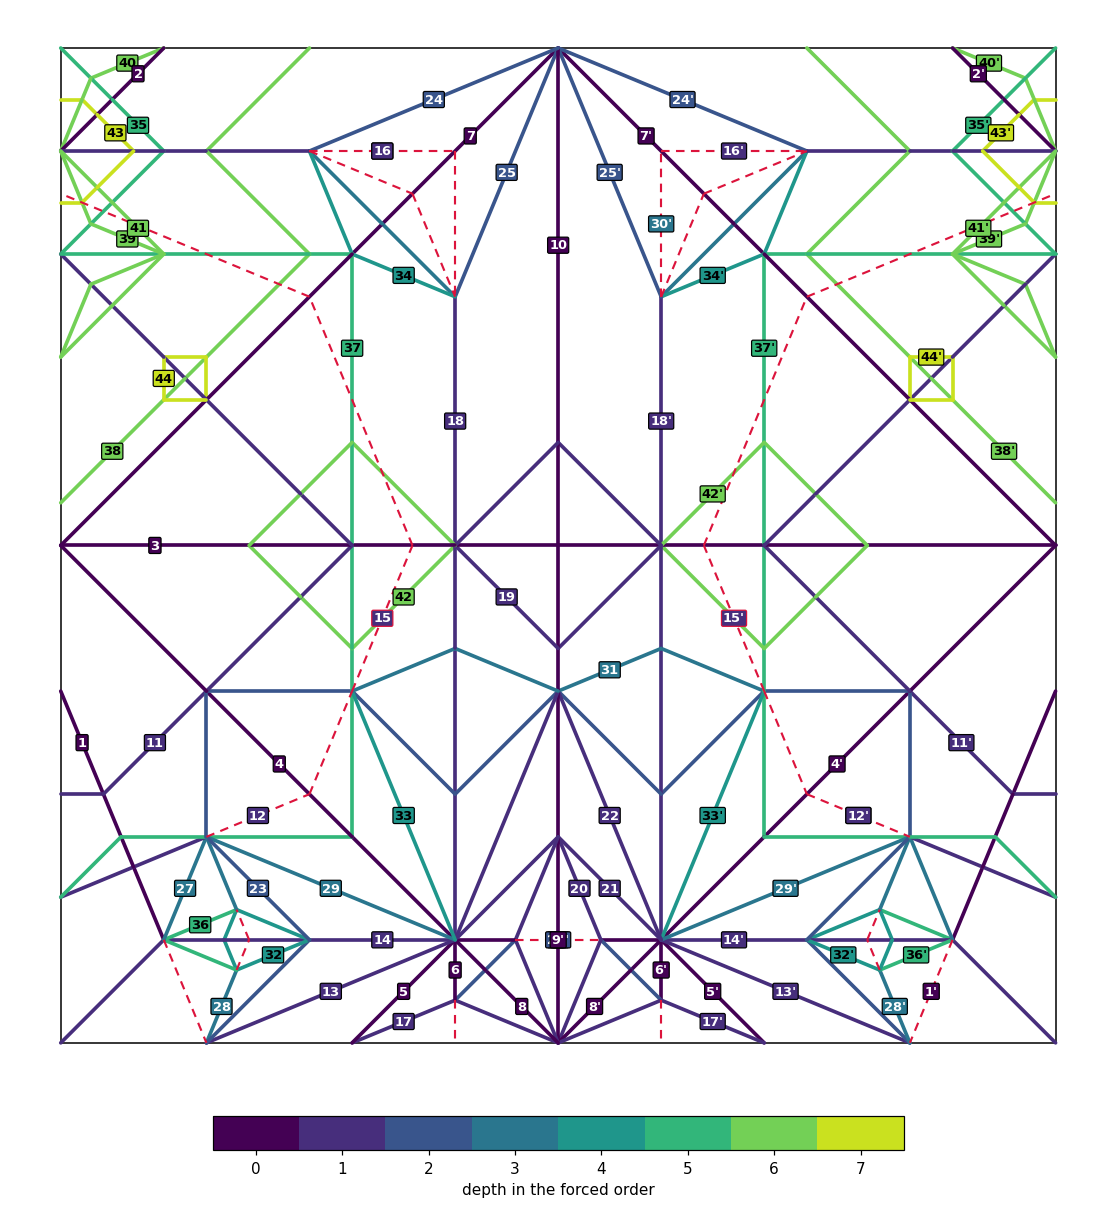
\includegraphics[height=0.44\textheight,keepaspectratio]{dragon_folds_c.png}\\[1mm]
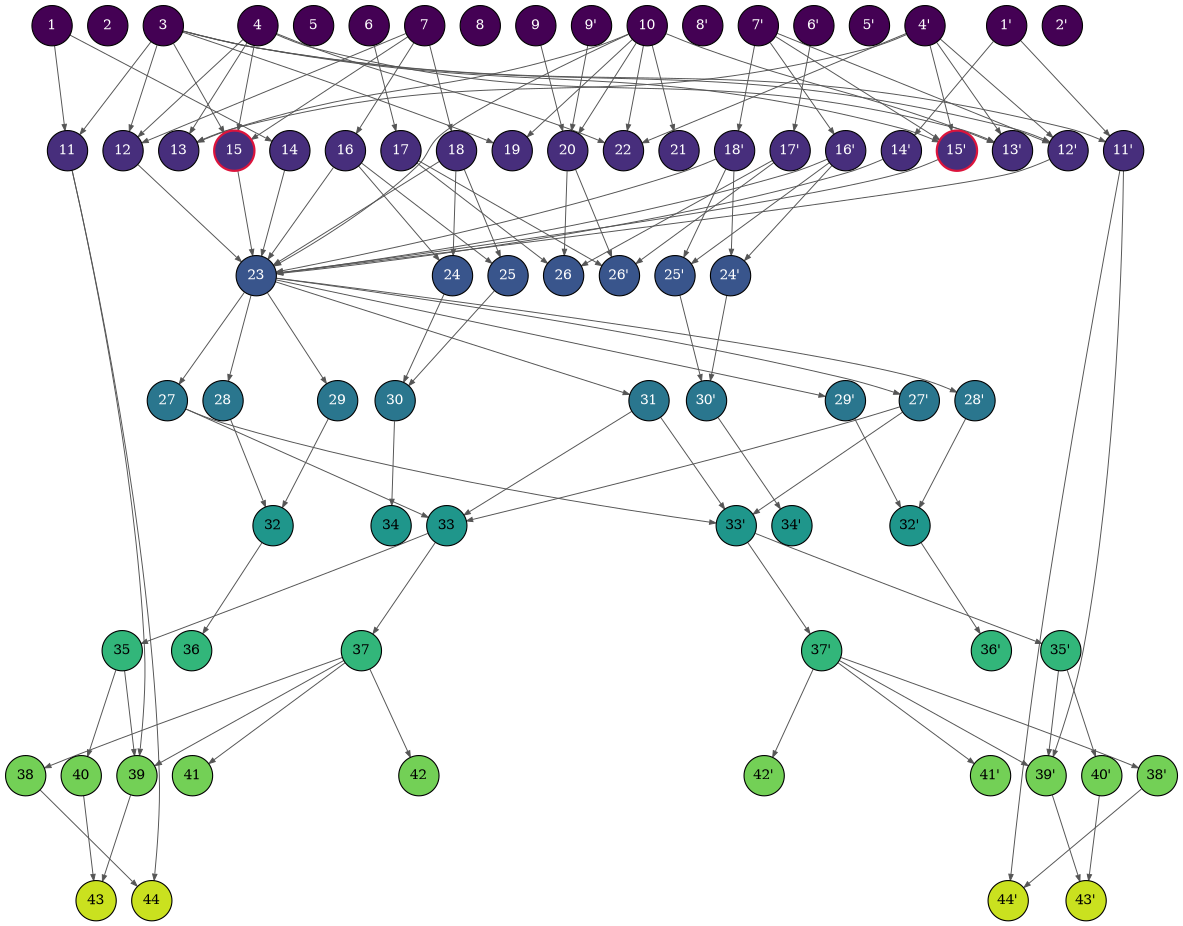
\includegraphics[width=\textwidth,height=0.42\textheight,keepaspectratio]{dragon_hasse.png}
\caption{Gentle Dragon. Top: the $80$ folds, coloured by depth in the forced order and labelled as in the Hasse diagram below; dashed crimson segments are cancelled; a prime marks the mirror image of a fold. Bottom: the Hasse diagram of the forced order. Each node is placed horizontally by its position on the sheet and vertically by its depth; crimson outlines mark folds made only of cancelled creases.}
\label{fig:dragon}
\end{figure}

\section{A corpus}\label{sec:corpus}

We ran the computation on $48$ patterns from the collection distributed with the flat-folder program~\cite{flatfolder}, with a budget of a few minutes per pattern on one core. The patterns were chosen to be small or medium-sized and varied: traditional bases and models, designs by Komatsu, Ku, Tanaka, Tachi, Furuta and others, tessellation-like patterns, and gadgets from hardness proofs~\cite{bernhayes,boxhard}. Table~\ref{tab:corpus} groups them by what their resolution needed.

{\small
\begin{longtable}{rl r r r r}
\caption{The corpus. ``Unit'' is the angular unit $2\pi/N$ when one fits, and --- when directions are kept as real numbers. ``Hidden'' is the number of hidden rays and ``coll.'' the number of vertices made by a collapse, in the minimal resolution found. Numbers are those of the collection.}\label{tab:corpus}\\
\toprule
\# & Pattern & Interior & Unit & Hidden & Coll.\\
\endfirsthead
\toprule
\# & Pattern & Interior & Unit & Hidden & Coll.\\
\endhead
\midrule\multicolumn{6}{l}{\emph{no cancellations} (8)}\\
001 & Traditional, Sailboat & 9 & 45$^\circ$ & 0 & 0 \\
002 & Traditional, Kabuto & 3 & 22.5$^\circ$ & 0 & 0 \\
007 & Ku, Pinwheel Pockets & 4 & 45$^\circ$ & 0 & 0 \\
026 & Furuta, orihazuru & 54 & --- & 0 & 0 \\
043 & Ku, Quad Overlap & 0 & 90$^\circ$ & 0 & 0 \\
074 & Miura, Miura-ori & 49 & 45$^\circ$ & 0 & 0 \\
301 & boxhard, Assigned Crossover & 16 & 90$^\circ$ & 0 & 0 \\
317 & boxhard, Unassigned Crossover & 4 & 90$^\circ$ & 0 & 0 \\
\midrule\multicolumn{6}{l}{\emph{cancellations at vertices with no single-line history} (20)}\\
004 & Traditional, Crane & 48 & 11.25$^\circ$ & 4 & 0 \\
006 & Ku, Thirds Pinwheel & 4 & 45$^\circ$ & 4 & 0 \\
038 & Traditional, Yakko & 16 & 45$^\circ$ & 6 & 0 \\
040 & Komatsu, Gentle Dragon & 103 & 22.5$^\circ$ & 24 & 0 \\
045 & Traditional, Pig & 21 & --- & 4 & 0 \\
052 & Traditional, House & 4 & 45$^\circ$ & 2 & 0 \\
056 & Tachi, Hoodman & 25 & 45$^\circ$ & 2 & 0 \\
062 & Furuta, houou & 24 & --- & 2 & 0 \\
067 & Traditional, damashi bune & 4 & 45$^\circ$ & 2 & 0 \\
073 & Komatsu, Squirrel & 33 & 22.5$^\circ$ & 22 & 0 \\
082 & Traditional, 4 Birdbase & 25 & 22.5$^\circ$ & 16 & 0 \\
089 & Traditional, 9 Birdbase & 69 & 22.5$^\circ$ & 24 & 0 \\
093 & Ku, 4 Stripes 3 & 36 & --- & 5 & 0 \\
102 & Traditional, Pinwheel & 4 & 45$^\circ$ & 4 & 0 \\
113 & Komatsu, Fox & 33 & 22.5$^\circ$ & 8 & 0 \\
114 & Kei, Kirby & 20 & 22.5$^\circ$ & 16 & 0 \\
141 & Kei, kitsune & 21 & 22.5$^\circ$ & 17 & 0 \\
244 & Komatsu, Smallbird Base & 3 & 22.5$^\circ$ & 2 & 0 \\
316 & boxhard, Unassigned Clause & 3 & 45$^\circ$ & 1 & 0 \\
318 & boxhard, Unassigned Split & 3 & 45$^\circ$ & 2 & 0 \\
\midrule\multicolumn{6}{l}{\emph{cancellations also at vertices that have one} (10)}\\
016 & Tanaka, enarc-crane final & 70 & 11.25$^\circ$ & 13 & 0 \\
035 & Tachi, kamehameha & 46 & 45$^\circ$ & 3 & 0 \\
058 & Ku, Color-change Pinwheel 1 & 16 & 22.5$^\circ$ & 16 & 0 \\
070 & Ku, Pygmy Jerboa & 46 & 22.5$^\circ$ & 9 & 0 \\
091 & Ku, 4 Stripes 1 & 14 & 22.5$^\circ$ & 6 & 0 \\
096 & Komatsu, Horned Owl & 20 & 22.5$^\circ$ & 16 & 0 \\
186 & Kei, Sus & 18 & 22.5$^\circ$ & 8 & 0 \\
292 & Tanaka, Aperiodic Monotile 1 & 10 & 30$^\circ$ & 5 & 0 \\
302 & boxhard, Assigned Clause & 23 & 45$^\circ$ & 16 & 0 \\
303 & boxhard, Assigned Split & 22 & 45$^\circ$ & 6 & 0 \\
\midrule\multicolumn{6}{l}{\emph{collapses} (4)}\\
015 & Ku, Iso-Area Half Square & 10 & --- & 0 & 6 \\
054 & Tanaka, Hexagon & 34 & 7.5$^\circ$ & 6 & 2 \\
084 & Ku, 4x4 Checkerboard & 20 & --- & 14 & 2 \\
325 & Bern--Hayes, Unassigned 45$^\circ$ Crossover & 4 & --- & 0 & 4 \\
\midrule\multicolumn{6}{l}{\emph{unresolved within the time budget} (6)}\\
018 & Komatsu, Butterfly Base & 49 & 22.5$^\circ$ & \multicolumn{2}{l}{} \\
030 & Tanaka, fish base & 62 & 11.25$^\circ$ & \multicolumn{2}{l}{} \\
048 & Komatsu, Dutch Rabbit & 27 & 22.5$^\circ$ & \multicolumn{2}{l}{} \\
055 & Komatsu, Sheep & 51 & 22.5$^\circ$ & \multicolumn{2}{l}{} \\
304 & boxhard, Assigned Solvable &  &  & \multicolumn{2}{l}{} \\
315 & Kei, Marnie & 24 & 22.5$^\circ$ & \multicolumn{2}{l}{} \\
\bottomrule
\end{longtable}
}

Several patterns show the parts of the method at work:
\begin{itemize}
\item \emph{Real directions.} The traditional pig uses $\arctan\frac12$ and $\arctan\frac13$, and Ku's $4\times4$ checkerboard uses $\arctan\frac13$; neither has an angular unit. The aperiodic monotiles use multiples of $30^\circ$.
\item \emph{Several hidden rays at one vertex.} The Horned Owl and Kirby need three or more at single vertices.
\item \emph{Hidden rays at vertices that have histories.} Ku's 4 Stripes 1, Color-change Pinwheel and the assigned split and clause gadgets of~\cite{boxhard} need cancelled segments through vertices whose own histories need none; the conflict analysis finds them.
\item \emph{Collapses.} The crossover gadget and Ku's Iso-Area Half Square need collapses, as do Tanaka's Hexagon and the checkerboard at two vertices each.
\end{itemize}

Of the six unresolved patterns, one has more than fifteen thousand vertices. In Tanaka's fish base, the conflicts returned at each round involve $4$ to $19$ vertices, and expanding all of them makes each round slower than the last. The others, Komatsu's Butterfly Base, Dutch Rabbit and Sheep and Morisue's Marnie, exceed the budget for reasons we have not isolated.

\section{Open problems}\label{sec:open}

\begin{enumerate}
\item \emph{Collapses.} Question~\ref{q:collapse}: does every flat vertex have a local history with cancellations using single-line steps only? The crossover gadget is the smallest test case. A negative answer would make collapses a necessary kind of move rather than a convenience.
\item \emph{Cancelled segments without a bend limit.} A cancelled segment's path is determined by the order: by Lemma~\ref{lem:crossing} it reflects at every earlier crease it meets and passes every later one. Tracing the path implied by the current solution, and refuting it if it does not close up, would remove restriction~1 of Section~\ref{sec:space} without enumerating paths. Restriction~2 can be removed in the same way, by adding the passing segment's hidden rays to the history at $w$.
\item \emph{From folds to moves.} Two folds made by one move are both mapped onto the move's fold line by the folding map at that moment. Since the folding map at any time is determined by the creases present, this is a global test for merging folds into moves, and the method does not yet use it.
\item \emph{Layers and colour.} Condition (C) is the only physical constraint used. Computing the order of layers in each intermediate state would turn resolutions into certificates and would predict the mountain and valley labels, which the method now ignores.
\item \emph{Benchmarks.} The fish base is a search problem: shrinking each conflict to a minimal one before expanding is the obvious next step. Komatsu's Butterfly Base and Morisue's Marnie are small enough that they should be resolvable, and finding out why they are not would test restrictions~1 and~2.
\end{enumerate}

\begin{thebibliography}{9}
\bibitem{akitaya13} H.~A. Akitaya, J.~Mitani, Y.~Kanamori, Y.~Fukui, Generating folding sequences from crease patterns of flat-foldable origami, ACM SIGGRAPH 2013 Posters.
\bibitem{boxhard} H.~A. Akitaya, K.~C. Cheung, E.~D. Demaine, T.~Horiyama, T.~C. Hull, J.~S. Ku, T.~Tachi, R.~Uehara, Box pleating is hard, in: Discrete and Computational Geometry and Graphs (JCDCG$^2$ 2015), LNCS 9943, Springer, 2016, 167--179.
\bibitem{arkin} E.~M. Arkin, M.~A. Bender, E.~D. Demaine, M.~L. Demaine, J.~S.~B. Mitchell, S.~Sethia, S.~S. Skiena, When can you fold a map?, Computational Geometry 29 (2004), 23--46.
\bibitem{bernhayes} M.~Bern, B.~Hayes, The complexity of flat origami, Proc.\ 7th ACM--SIAM Symposium on Discrete Algorithms (1996), 175--183.
\bibitem{z3} L.~de Moura, N.~Bj{\o}rner, Z3: an efficient SMT solver, TACAS 2008, LNCS 4963, 337--340.
\bibitem{demaine} E.~D. Demaine, J.~O'Rourke, Geometric Folding Algorithms: Linkages, Origami, Polyhedra, Cambridge University Press, 2007.
\bibitem{hull} T.~Hull, On the mathematics of flat origamis, Congressus Numerantium 100 (1994), 215--224.
\bibitem{flatfolder} J.~S. Ku, Flat-Folder, software and example collection, \url{https://github.com/origamimagiro/flat-folder}.
\end{thebibliography}

\appendix
\section{The vertices of the running pattern}\label{app:table}

For each interior vertex of the running pattern, the table gives its coordinates, the directions of its rays in units of $\pi/32$ (with $0,0$ for the two hidden creases at $\vstar$), and its local histories, written as sequences of folds. Where a vertex has several histories they are separated by semicolons; the global order selects among them.

{\small
\begin{longtable}{l l l}
\toprule
vertex & directions & local histories\\
\midrule
\endhead
$(4.000, 6.343)$ & 4, 10, 16, 36, 56, 62 & $P_1^{+}$ $\to$ $C'$ $\to$ $C$; $P_1^{+}$ $\to$ $C$ $\to$ $C'$ \\
$(1.313, 6.000)$ & 0, 16, 32, 48 & $A^{+}$ $\to$ $E$; $E$ $\to$ $A^{+}$ \\
$(1.920, 6.000)$ & 0, 19, 32, 45 & $A^{+}$ $\to$ $E'$ \\
$(3.172, 6.000)$ & 0, 4, 32, 60 & $A^{+}$ $\to$ $P_1^{+}$ \\
$(4.343, 6.000)$ & 0, 24, 32, 40 & $A^{+}$ $\to$ $C$ \\
$(5.725, 6.000)$ & 0, 30, 32, 34 & $A^{+}$ $\to$ $C'$ \\
$(6.000, 6.000)$ & 0, 8, 32, 56 & $A^{+}$ $\to$ $P_2^{+}$ \\
$(7.172, 6.000)$ & 0, 12, 32, 52 & $A^{+}$ $\to$ $P_3^{+}$ \\
$(7.293, 5.707)$ & 4, 20, 36, 52 & $I$ $\to$ $P_3^{+}$; $P_3^{+}$ $\to$ $I$ \\
$(4.000, 5.657)$ & 2, 8, 28, 48, 54, 60 & $P_1^{+}$ $\to$ $C'$ $\to$ $C$; $P_1^{+}$ $\to$ $C$ $\to$ $C'$ \\
$(6.586, 5.414)$ & 4, 24, 44, 56 & $P_2^{+}$ $\to$ $I$ \\
$(6.293, 4.707)$ & 12, 28, 44, 60 & $I$ $\to$ $P_1^{+}$; $P_1^{+}$ $\to$ $I$ \\
$(1.313, 4.000)$ & 0, 13, 16, 32, 48, 51 & $A^{0}$ $\to$ $E$ $\to$ $E'$; $A^{0}$ $\to$ $E'$ $\to$ $E$; $E$ $\to$ $A^{0}$ $\to$ $E'$ \\
$(4.000, 4.000)$ & 0, 16, 32, 48 & $A^{0}$ $\to$ $C$; $C$ $\to$ $A^{0}$ \\
$(5.107, 4.000)$ & 0, 22, 32, 42 & $A^{0}$ $\to$ $C'$ \\
$(6.000, 4.000)$ & 0, 0, 12, 32, 40, 52 & $A^{0}$ $\to$ $I$ $\to$ $F$ \\
$(6.293, 3.293)$ & 4, 20, 36, 52 & $I$ $\to$ $P_1^{-}$; $P_1^{-}$ $\to$ $I$ \\
$(4.586, 2.586)$ & 0, 4, 8, 36 & $P_1^{-}$ $\to$ $F$ \\
$(6.586, 2.586)$ & 8, 20, 32, 40, 48, 60 & $P_2^{-}$ $\to$ $F$ $\to$ $I$; $P_2^{-}$ $\to$ $I$ $\to$ $F$ \\
$(4.000, 2.343)$ & 4, 10, 16, 36, 56, 62 & $P_1^{-}$ $\to$ $C$ $\to$ $C'$; $P_1^{-}$ $\to$ $C'$ $\to$ $C$ \\
$(7.293, 2.293)$ & 12, 28, 44, 60 & $P_3^{-}$ $\to$ $I$; $I$ $\to$ $P_3^{-}$ \\
$(1.313, 2.000)$ & 0, 16, 32, 48 & $E$ $\to$ $A^{-}$; $A^{-}$ $\to$ $E$ \\
$(1.920, 2.000)$ & 0, 19, 32, 45 & $A^{-}$ $\to$ $E'$ \\
$(3.172, 2.000)$ & 0, 4, 32, 60 & $A^{-}$ $\to$ $P_1^{-}$ \\
$(4.343, 2.000)$ & 0, 24, 32, 40 & $A^{-}$ $\to$ $C$ \\
$(5.725, 2.000)$ & 0, 30, 32, 34 & $A^{-}$ $\to$ $C'$ \\
$(6.000, 2.000)$ & 0, 8, 32, 56 & $A^{-}$ $\to$ $P_2^{-}$ \\
$(6.586, 2.000)$ & 0, 16, 32, 48 & $F$ $\to$ $A^{-}$; $A^{-}$ $\to$ $F$ \\
$(7.172, 2.000)$ & 0, 12, 32, 52 & $A^{-}$ $\to$ $P_3^{-}$ \\
$(4.000, 1.657)$ & 2, 8, 28, 48, 54, 60 & $P_1^{-}$ $\to$ $C$ $\to$ $C'$; $P_1^{-}$ $\to$ $C'$ $\to$ $C$ \\
$(4.586, 1.414)$ & 0, 28, 56, 60 & $P_1^{-}$ $\to$ $F$ \\
$(6.586, 1.414)$ & 16, 24, 32, 56 & $P_2^{-}$ $\to$ $F$ \\
\bottomrule
\end{longtable}
}

\end{document}
